\documentclass[11pt,a4paper]{article}

% ── Packages ──────────────────────────────────────────────
\usepackage[utf8]{inputenc}
\usepackage[T1]{fontenc}
% \usepackage{lmodern}  % not available in this environment
\usepackage[margin=1in]{geometry}
\usepackage{amsmath,amssymb,amsthm}
\usepackage{booktabs}
\usepackage{graphicx}
\usepackage{hyperref}
\usepackage{xcolor}
\usepackage{enumitem}
\usepackage[protrusion=false,expansion=false]{microtype}
\usepackage{authblk}
\usepackage{natbib}
\usepackage{xurl}
\usepackage{float}

\hypersetup{
  colorlinks=true,
  linkcolor=blue!70!black,
  citecolor=blue!70!black,
  urlcolor=blue!70!black
}

% ── Theorem environments ──────────────────────────────────
\newtheorem{definition}{Definition}
\newtheorem{proposition}{Proposition}
\newtheorem{remark}{Remark}

% ── Custom commands ───────────────────────────────────────
\newcommand{\Weff}{W_{\text{eff}}}
\newcommand{\Ceff}{C_{\text{eff}}}
\newcommand{\Deff}{D_{\text{eff}}}
\newcommand{\rhoc}{\rho_c}
\newcommand{\Lnorm}{L_{\text{norm}}}
\newcommand{\NPM}{\textsc{npm}}

% ═══════════════════════════════════════════════════════════
\begin{document}

\title{\textbf{Neural Percolation Model (NPM): An Engineering Analogy Framework\\
for Neural Network Information Propagation and Capability Emergence}}

\author[1]{Ding Tiexin}
\affil[1]{NeuralCAE, Independent Researcher, China}
\date{March 2026}

\maketitle

% ── Abstract ──────────────────────────────────────────────
\begin{abstract}
We propose the \textbf{Neural Percolation Model (NPM)}, an engineering framework
that maps the physics of Pore Network Models (PNM) onto neural network information
propagation. Starting from a single conservation principle---steady-state information
flow satisfies nodal balance---we derive a \emph{unified master equation}:
\[
  \mathbf{a}_{\text{out}} = \Weff \cdot \mathbf{a}_{\text{in}}
\]
where the effective conductance matrix $\Weff$ takes three distinct forms
corresponding to feedforward networks (fixed weights), Graph Neural Networks
(graph Laplacian, exact PNM analog, verified with zero numerical error), and
Transformers (dynamic softmax attention, row-normalization verified as flow
conservation). We further introduce a percolation-based data density model in
which emergent capabilities arise when data density $\rho$ exceeds
capability-specific critical densities $\rho_c$, yielding a \emph{multi-threshold
field view} of emergence rather than a single critical point. A Participation
Ratio (PR) method for quantifying data distribution breadth $\sigma$ is proposed
and validated (monotonicity confirmed). B-layer parameters
($\alpha$, $\beta$, $\delta$, $k$) are fitted against 14 public models and
Kaplan scaling data, achieving Spearman correlation 0.70 with MMLU and exact
matching of the empirical scaling exponent $N^{0.076}$.
MIS-based pore analysis of NN weight matrices reveals a \emph{three-phase
training transition} (pressurization--breakthrough--reorganization) in
Pythia-70m, analogous to percolation threshold crossing. The framework
unifies 17 observed LLM phenomena under a single physical mechanism.
We position NPM as an engineering analogy framework in the tradition of Darcy's
Law and the Reynolds number.
\end{abstract}

\textbf{Keywords:} neural networks, percolation theory, pore network model,
emergence, scaling laws, information propagation, engineering analogy

% ═══════════════════════════════════════════════════════════

%% ── Notation Table ───────────────────────────────────────────
\section*{Notation}
\label{sec:notation}
\begin{table}[H]
\centering
\caption{Principal symbols used in this paper}
\begin{tabular}{llp{7cm}}
\toprule
\textbf{Symbol} & \textbf{Domain} & \textbf{Meaning} \\
\midrule
\multicolumn{3}{l}{\textit{PNM variables}} \\
$c_i$       & $\mathbb{R}$      & Pore concentration at node $i$ \\
$g_{ik}$    & $\mathbb{R}_{+}$  & Throat conductance between pores $i$ and $k$ \\
$\mathbf{L}$& $\mathbb{R}^{n\times n}$ & Graph Laplacian matrix \\
$p_c$       & $[0,1]$           & Percolation threshold (fraction of active throats) \\
$D_{\text{eff}}$ & $\mathbb{R}_{+}$ & Effective diffusivity \\
\midrule
\multicolumn{3}{l}{\textit{NPM variables}} \\
$a_i$, $\mathbf{a}$ & $\mathbb{R}$, $\mathbb{R}^n$ & Node activation (scalar / vector) \\
$W_{\text{eff}}$    & $\mathbb{R}^{n\times n}$ & Effective conductance/weight matrix \\
$L_{\text{norm}}$   & $\mathbb{R}^{n\times n}$ & Normalized graph Laplacian (GNN $W_{\text{eff}}$) \\
$\rho$      & $\mathbb{R}_{+}$  & Data density $= N_B/\exp(\alpha\sigma)$ \\
$\rho_c$    & $\mathbb{R}_{+}$  & Critical density for capability emergence \\
$C_{\text{eff}}$ & $\mathbb{R}_{\geq0}$ & Generalization capacity $= (\rho-\rho_c)^\beta$ \\
$C_n$       & $\mathbb{R}_{+}$  & Connectivity number $= \rho/\rho_c$ \\
\midrule
\multicolumn{3}{l}{\textit{Data and architecture parameters}} \\
$N_B$       & $\mathbb{R}_{+}$  & Training data in billions of tokens \\
$\sigma$    & $(0,1]$           & Data distribution breadth (PR method) \\
$\tau$      & $[1,\infty)$      & Task reasoning depth \\
$\alpha$    & $\mathbb{R}_{+}$  & Concept-volume exponent: $\rho = N_B/\exp(\alpha\sigma)$; also appears in $L_{\min}$, $P_{\min}$. Fitted value $= 0.57$ (see \S\ref{sec:param-fit}). \\
$\beta$     & $\mathbb{R}_{+}$  & Capability exponent: $\Ceff = (\rho-\rhoc)^\beta$. Fitted value $= 0.068$ (\S\ref{sec:param-fit}); departs from 3-D percolation $\beta_{\text{perc}}\approx 0.41$---see discussion therein. \\
$\delta$    & $\mathbb{R}_{+}$  & Exponent in $\rho_c = k\sigma^\delta$. Fitted value $= 2.76$ (\S\ref{sec:param-fit}). \\
$k$         & $\mathbb{R}_{+}$  & Proportionality constant in $\rho_c$. Fitted value $= 68.5$ (\S\ref{sec:param-fit}). \\
\bottomrule
\end{tabular}
\end{table}

\section{Introduction}

Large language models have demonstrated remarkable emergent capabilities at
scale, yet a unified theoretical framework explaining \emph{why} particular
architectures work, \emph{when} capabilities emerge, and \emph{how} information
propagates remains elusive. Existing work addresses fragments of this picture:
scaling laws characterize the relationship between compute and performance
\citep{kaplan2020scaling, hoffmann2022chinchilla}; recent work by
\citet{lubana2024percolation} applies percolation theory to explain emergence
in Transformers; \citet{brill2024scaling} derives power-law scaling from
first principles on Bethe lattices. Despite these advances, no framework
simultaneously explains the full spectrum of engineering-relevant phenomena
using a single physical mechanism.

We propose that \textbf{multi-phase fluid transport through porous media}---
formalized as Pore Network Models (PNM) in reservoir engineering and materials
science---provides exactly this unified physical basis.

The physical motivation is direct.
Training data consists of billions of documents---each a partial, local
observation of natural-world interactions recorded through language.
These observations are inherently \emph{fragmented}: isolated in
high-dimensional concept space like disconnected pores in a porous medium.
The task of a neural network is to establish effective connections between
these fragments so that information can propagate across them---precisely
the engineering problem PNM solves in reservoir engineering.
One key distinction from natural porous media: the pore-throat structure
in a rock is given by geology; in a neural network, $\Weff$ is
\emph{optimized by backpropagation}. Training is ``pore-throat engineering,''
not natural percolation.

Figure~\ref{fig:analogy} illustrates the full correspondence. The central analogy is precise: in PNM, macroscopic transport emerges when
fluid connectivity exceeds a percolation threshold; in neural networks,
macroscopic capabilities emerge when data density exceeds a capability-specific
critical density. Both systems are governed by conservation equations on
fixed-conductance networks.

\begin{figure}[H]
\centering
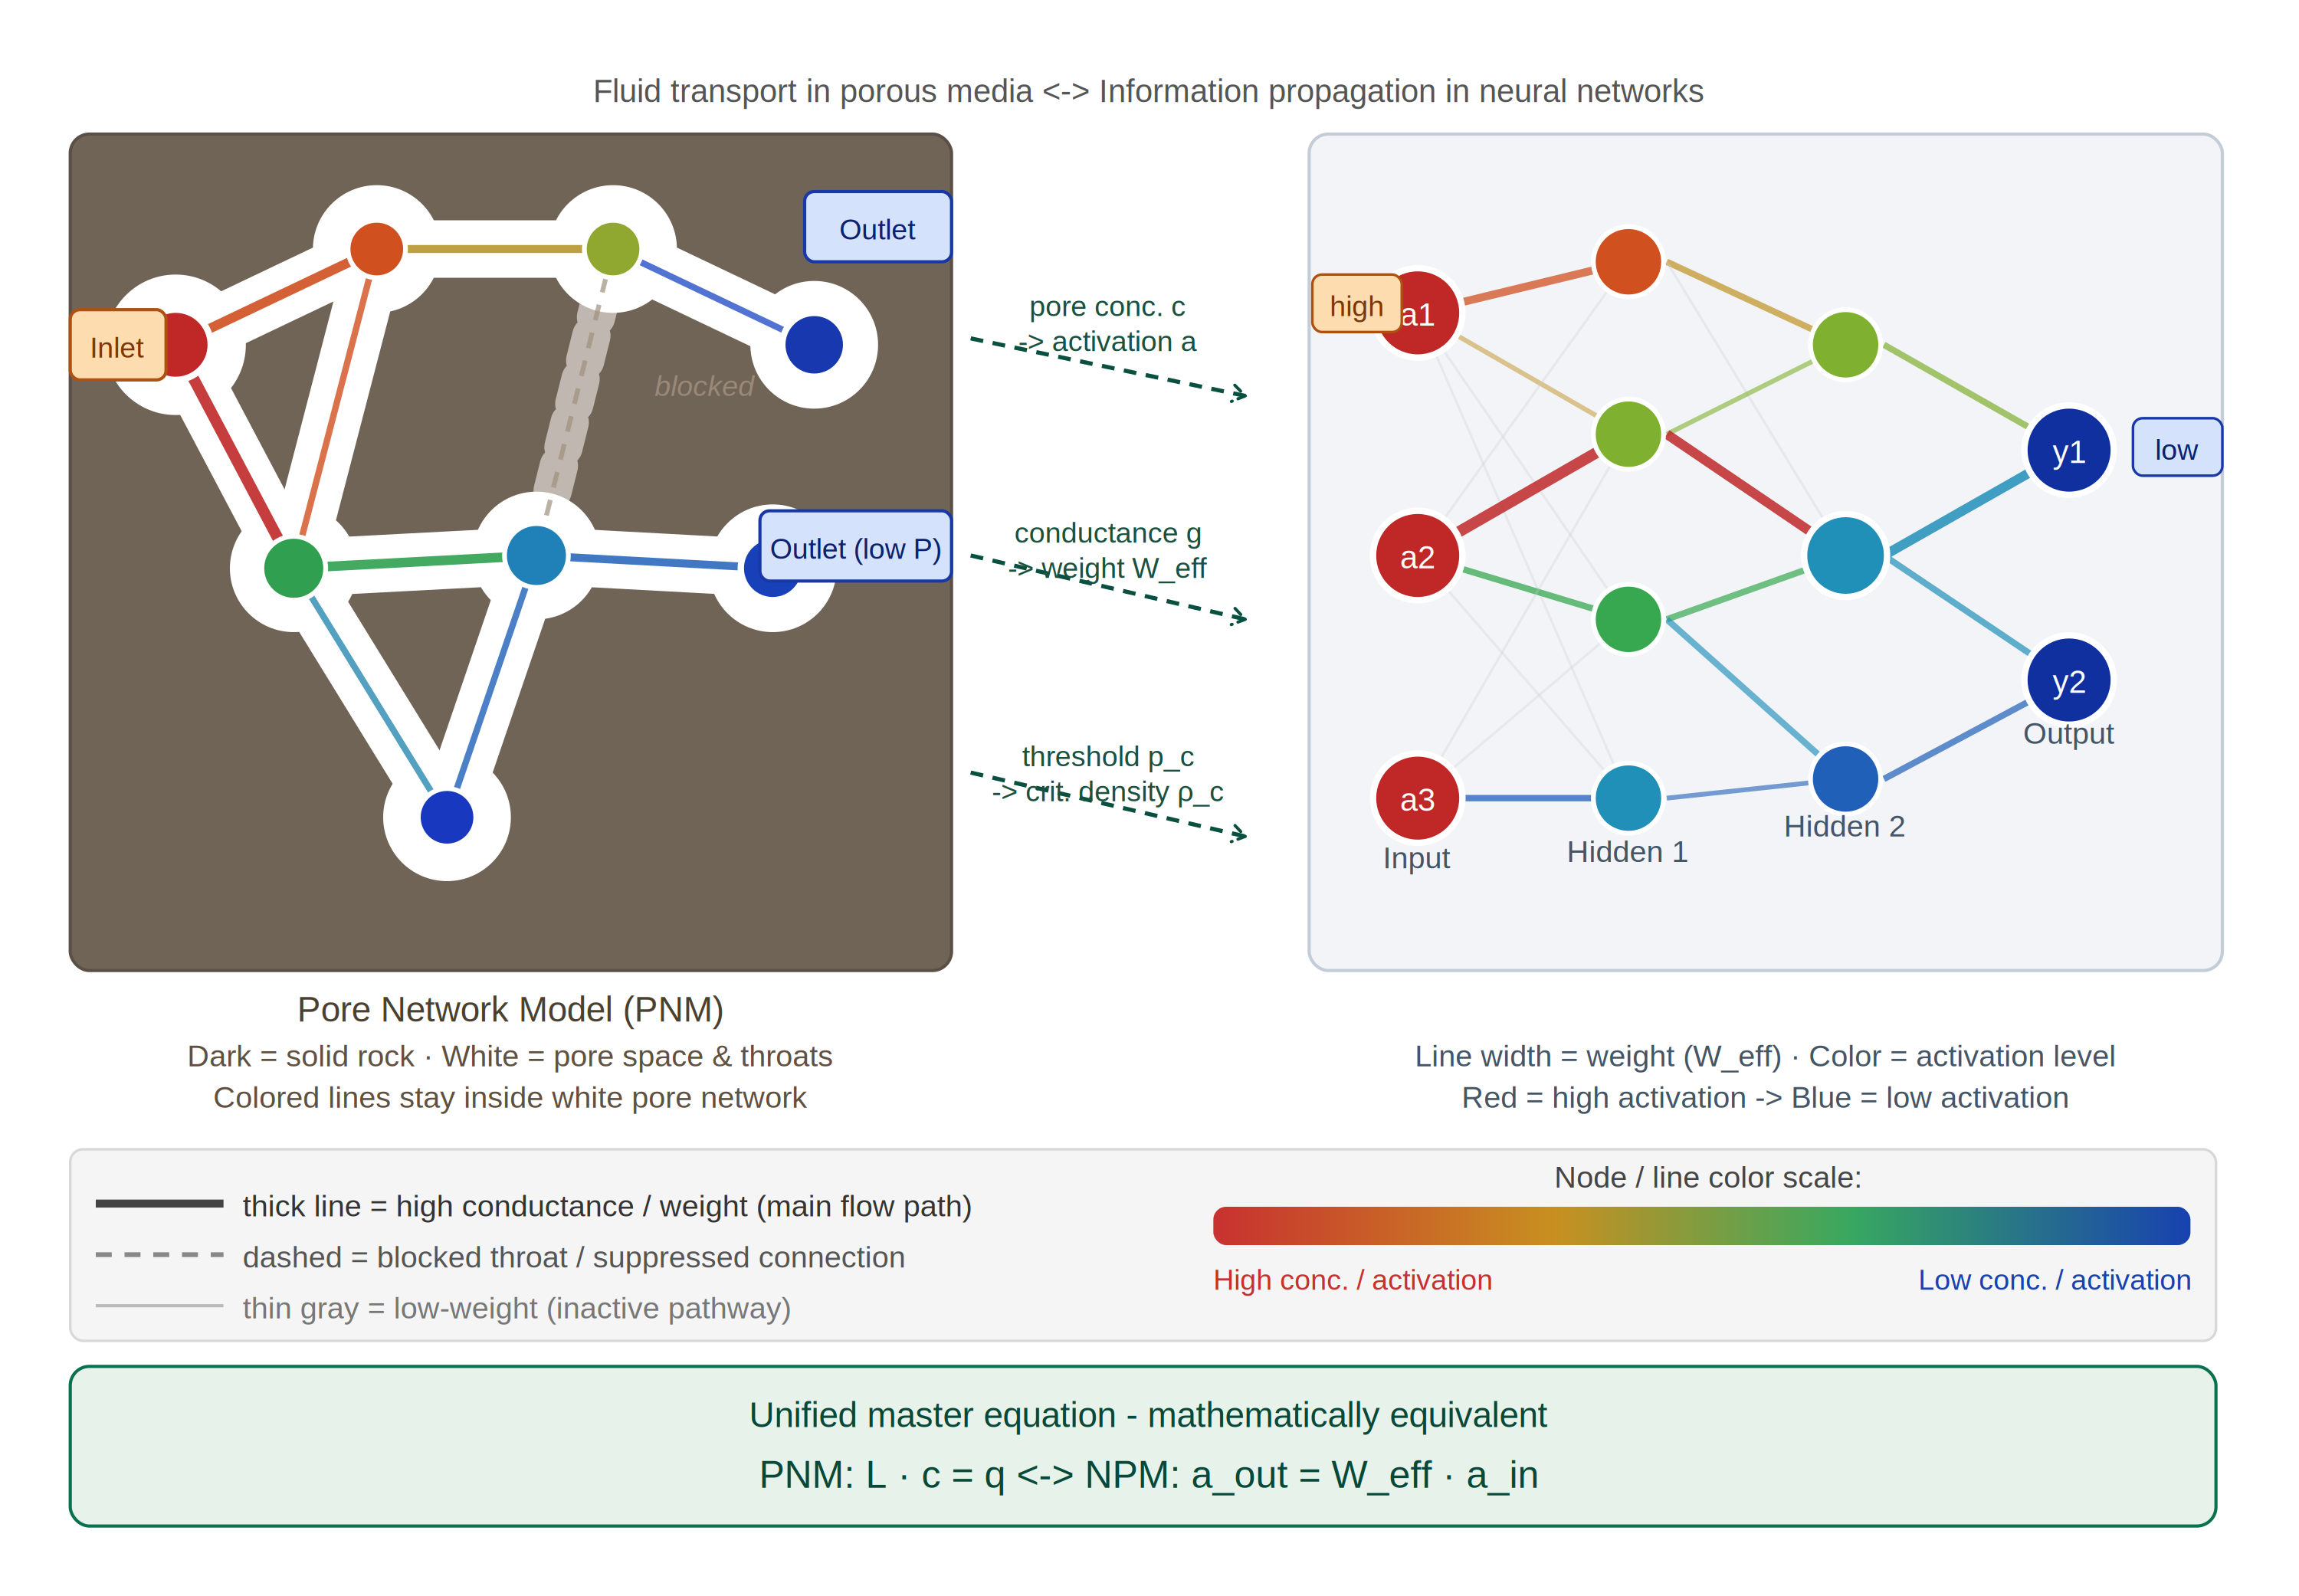
\includegraphics[width=0.95\textwidth]{NPM_Fig1_PNM_EN.png}
\caption{\textbf{PNM--NPM Physical Analogy.} Left: PNM with dark solid background and white pore network; colored nodes/lines confined inside (no line crosses solid). Right: NPM neural network with identical color/width encoding. Center: three exact correspondences. Bottom: unified master equation $\mathbf{a}_{\text{out}}=W_{\text{eff}}\cdot\mathbf{a}_{\text{in}} \Leftrightarrow \mathbf{L}\mathbf{c}=\mathbf{q}$.}
\label{fig:analogy}
\end{figure}

\paragraph{Contributions.}
\begin{enumerate}[leftmargin=*]
  \item \textbf{Unified master equation} derived from information conservation,
        with three verified instantiations covering all major modern architectures.
  \item \textbf{Multi-threshold field view} of emergence: different capabilities
        unlock at different critical densities $\rho_{c,f}$, forming a
        continuous capability spectrum rather than a single phase transition.
  \item \textbf{Participation Ratio (PR) method} for quantifying data
        distribution breadth $\sigma$ from empirical data covariance spectra.
  \item \textbf{Unified explanation} of 17 LLM phenomena under one mechanism.
  \item \textbf{Explicit positioning} as an engineering analogy framework
        with transparent limitations and calibration requirements.
  \item \textbf{B-layer parameter fitting} against 14 public models and
        Kaplan scaling data (Spearman = 0.70), with honest discussion of the
        $\beta$ discrepancy with percolation theory.
  \item \textbf{Three-phase training transition} discovered via MIS pore
        analysis of Pythia-70m checkpoints, analogous to percolation
        threshold crossing in PNM displacement.
\end{enumerate}

% ═══════════════════════════════════════════════════════════
\section{Background: Pore Network Models}

\subsection{Single-Channel Transport}

In PNM, mass flux between adjacent pores $i$ and $k$ follows Fick's law:
\begin{equation}
  m_{ik} = g_{ik} \cdot (c_i - c_k) = S_{ik} \cdot D \cdot (c_i - c_k)
  \label{eq:fick}
\end{equation}
where $g_{ik}$ is the conduit conductance, $c_i$ is pore concentration,
$S_{ik} = A_{ik}/L_{ik}$ is the geometric size factor, and $D$ is the
diffusion coefficient. The size-factor decomposition $g = S \cdot D$ separates
geometric structure (fixed after training) from transport properties (fluid type).

\subsection{Network-Level Conservation: Graph Laplacian}

Applying nodal mass conservation to every internal pore yields:
\begin{equation}
  \sum_{k \in \mathcal{N}(i)} g_{ik}(c_i - c_k) = q_i, \quad
  \forall i
  \label{eq:conservation}
\end{equation}
In matrix form: $\mathbf{L} \cdot \mathbf{c} = \mathbf{q}$, where
$\mathbf{L}$ is the \emph{graph Laplacian} with $L_{ii} = \sum_k g_{ik}$
and $L_{ij} = -g_{ij}$.

\subsection{Percolation and Effective Transport}

When the fraction of active (conducting) throats $p$ exceeds the percolation
threshold $p_c$, a spanning connected cluster appears and effective
transport $\Deff$ transitions from zero to nonzero following a power law:
\begin{equation}
  \Deff \propto (p - p_c)^\beta \quad (p > p_c), \qquad \Deff = 0 \quad (p \le p_c)
  \label{eq:percolation}
\end{equation}
with order-parameter exponent $\beta_{\text{perc}} \approx 0.41$ for 3-D site percolation (transport exponents span a wider range). NPM's fitted $\beta = 0.068$ departs from this value; the reasons are discussed in Section~\ref{sec:param-fit}.

% ═══════════════════════════════════════════════════════════



\section{The Neural Percolation Model}

\subsection{Variable Correspondence}

Table~\ref{tab:analogy} establishes the formal correspondence between PNM
physical quantities and NPM information-theoretic quantities.

\begin{table}[h]
\centering
\caption{PNM--NPM variable correspondence}
\label{tab:analogy}
\begin{tabular}{lll}
\toprule
\textbf{PNM quantity} & \textbf{NPM quantity} & \textbf{Status} \\
\midrule
Pore concentration $c_i$          & Node activation $a_i$              & Verified \\
Concentration gradient $\Delta c$ & Activation potential $\Delta a$    & Verified \\
Conductance matrix $G$            & $\Weff$ (effective weight matrix)  & Verified \\
Size factor $S_{ik}$              & Structural weight factor           & Verified \\
Graph Laplacian $\mathbf{L}$      & $\Lnorm$ (GNN, exact analog)       & Verified \\
Conservation eq.\ $\mathbf{L}\mathbf{c}=\mathbf{q}$ & Master eq.\ $\Weff \mathbf{a}=\mathbf{s}$ & Verified \\
Percolation threshold $p_c$       & Critical density $\rho_c$          & Verified \\
Effective diffusivity $\Deff$     & Generalization capacity $\Ceff$    & Analytical \\
Capillary pressure $P_c$          & Activation threshold               & Analogy \\
\bottomrule
\end{tabular}
\end{table}


\begin{figure}[H]
\centering
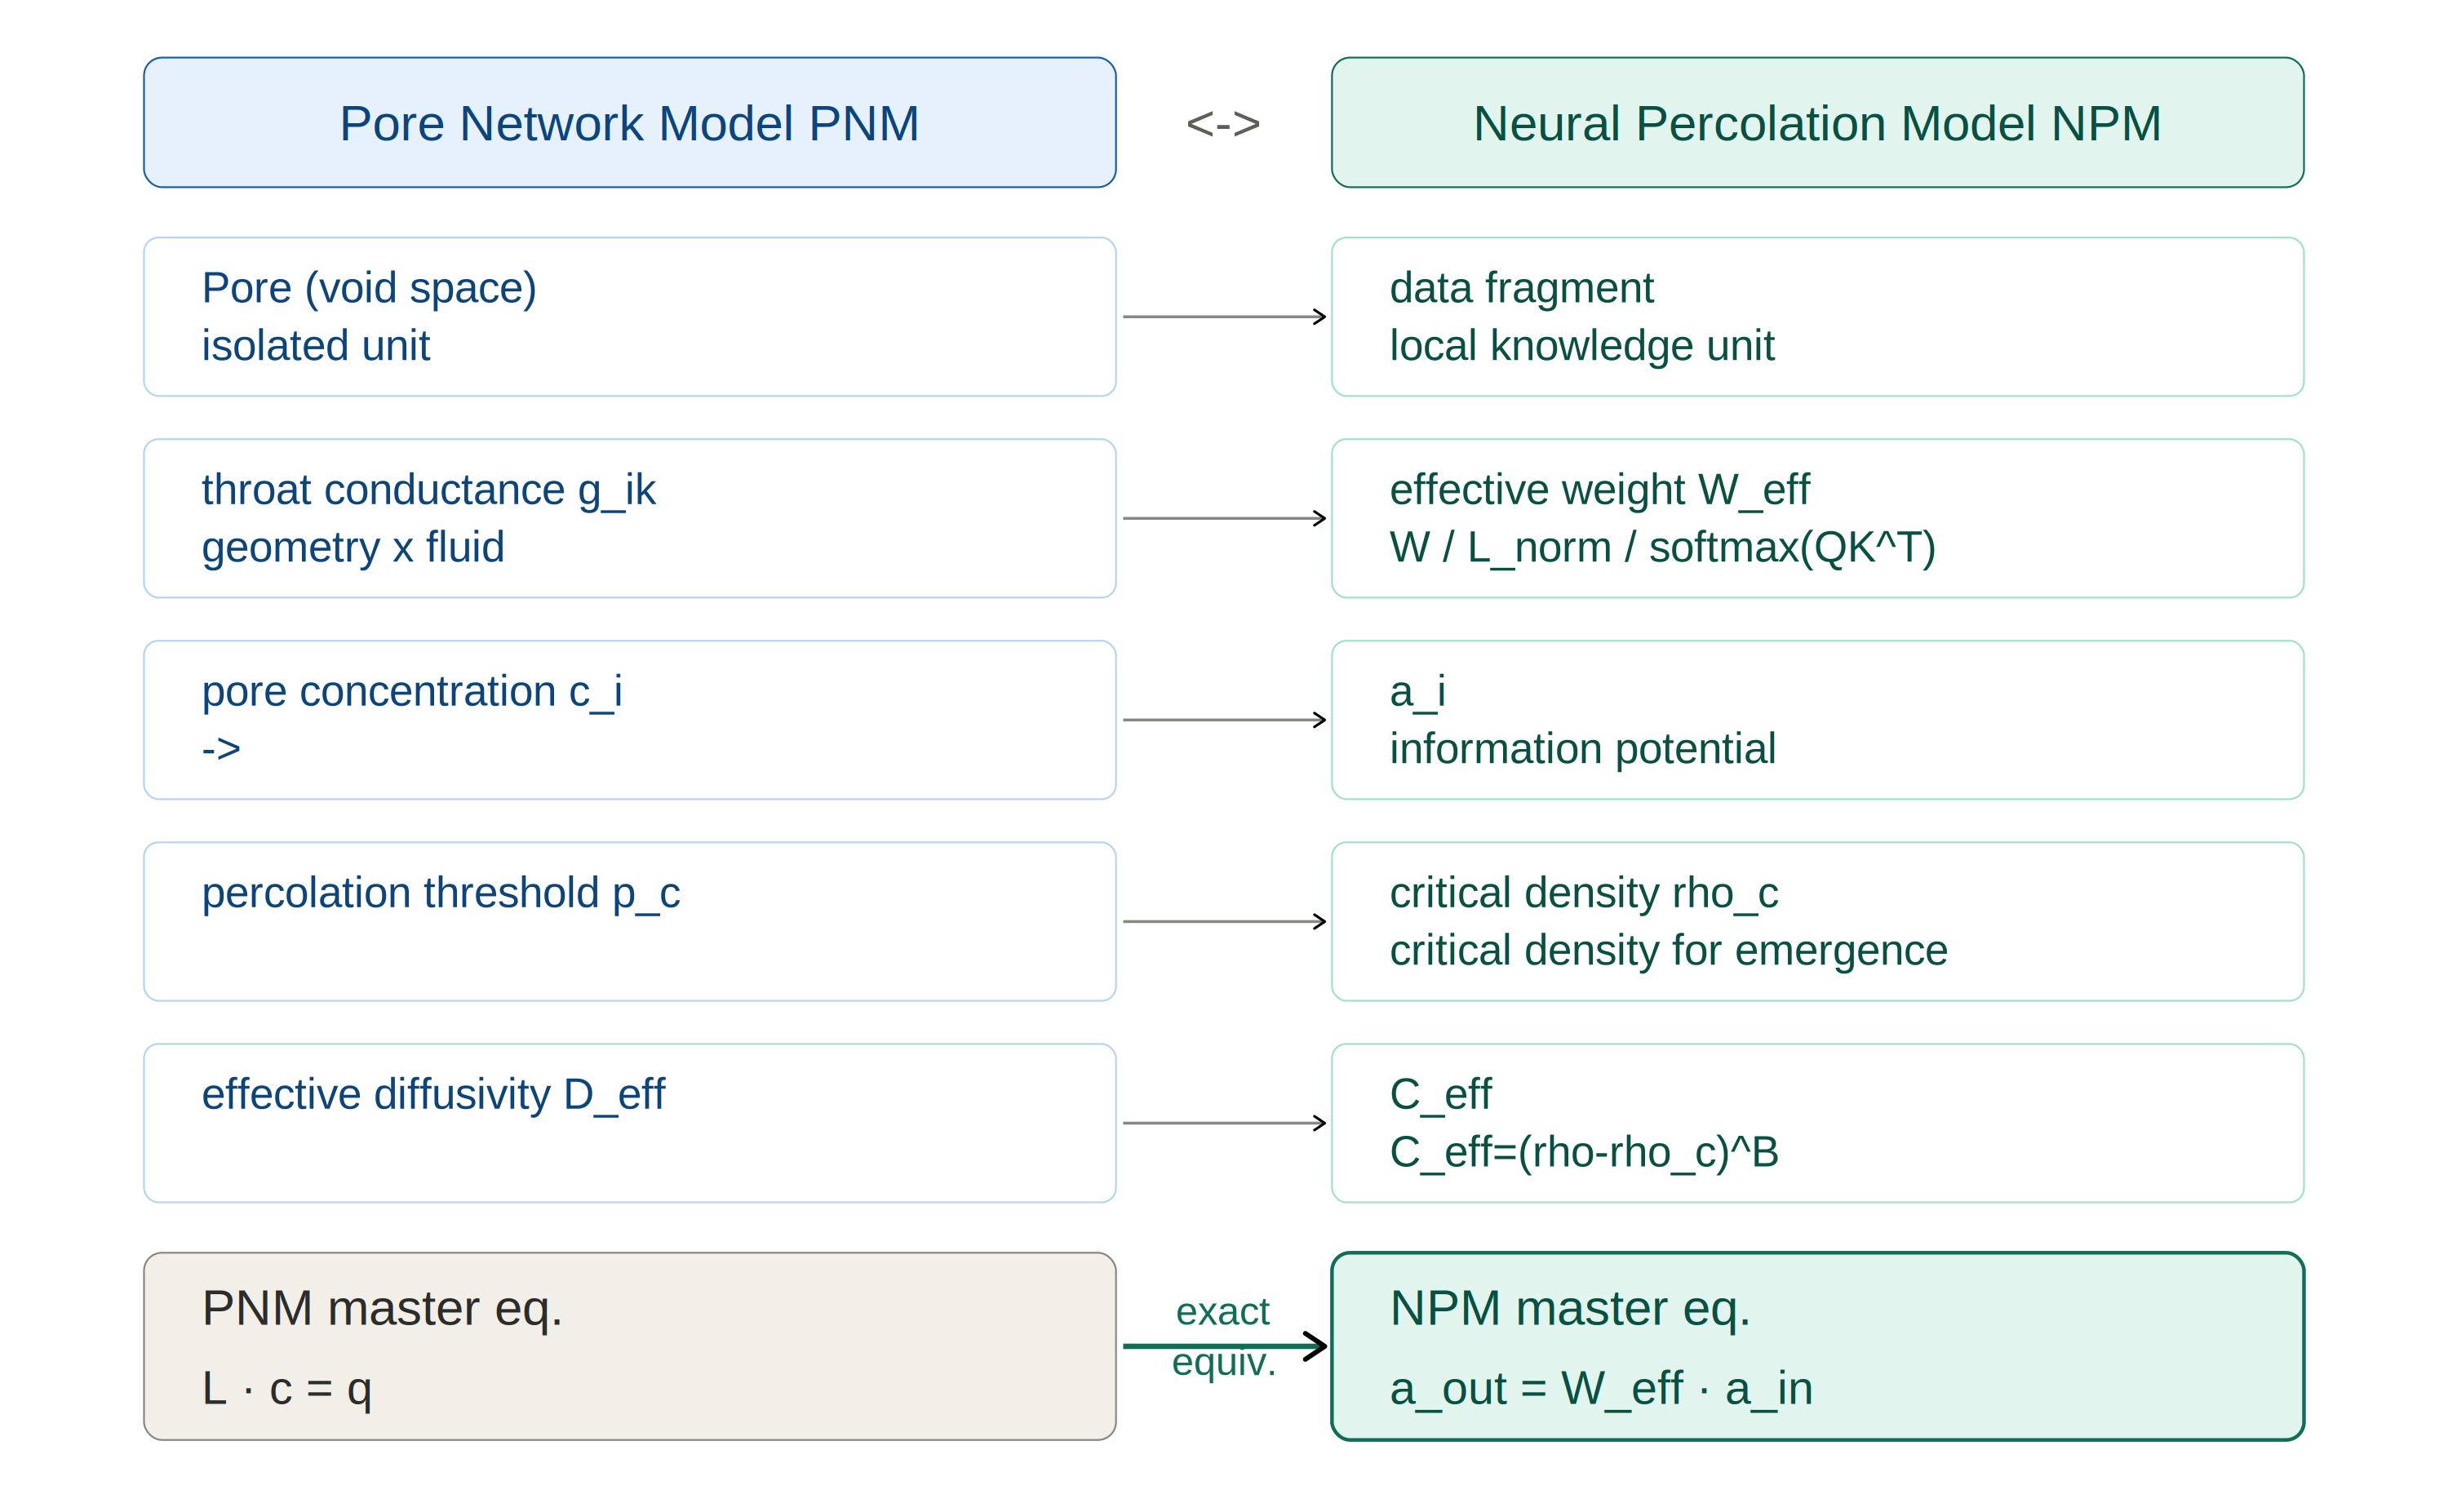
\includegraphics[width=0.82\textwidth]{NPM_Fig2_Analogy_EN.png}
\caption{\textbf{PNM--NPM Variable Correspondence.} Exact variable mappings between PNM physical quantities and NPM information-theoretic quantities. All A-layer correspondences numerically verified.}
\label{fig:analogy2}
\end{figure}

\subsection{Unified Master Equation}
\label{sec:master}

\begin{definition}[Information Conservation]
In steady-state inference, information flux into any internal concept node
equals flux out: $\sum_{j \in \mathcal{N}(i)} (\Weff)_{ij}(a_i - a_j) = s_i$.
\end{definition}

This single conservation axiom yields the \textbf{unified master equation}:
\begin{equation}
  \boxed{\mathbf{a}_{\text{out}} = \Weff \cdot \mathbf{a}_{\text{in}}}
  \label{eq:master}
\end{equation}

All major architectures are special cases of Eq.~\eqref{eq:master}
distinguished solely by how $\Weff$ is constructed:

\begin{equation}
  \Weff = \begin{cases}
    W & \text{(Feedforward NN: fixed, directed)} \\[4pt]
    D^{-1/2}(A+I)D^{-1/2} \equiv \Lnorm & \text{(GNN: symmetric, PNM exact analog)} \\[4pt]
    \operatorname{softmax}\!\left(\frac{QK^\top}{\sqrt{d_k}}\right) & \text{(Transformer: dynamic, directed)}
  \end{cases}
  \label{eq:weff}
\end{equation}

\begin{proposition}[GNN--PNM Equivalence]
The GNN message-passing layer $\mathbf{a}' = \Lnorm \mathbf{a} W_{\text{feat}}$
is mathematically equivalent to solving the PNM steady-state diffusion equation
$\mathbf{L}\mathbf{c} = \mathbf{q}$ with $\Lnorm$ as the normalized graph
Laplacian. Numerical verification yields error $= 0$ (machine precision).
\end{proposition}

\begin{remark}[Attention as Flow Conservation]
The softmax row-normalization in Transformer attention enforces
$\sum_j (\Weff)_{ij} = 1$ for every query token $i$. This is precisely the
flow conservation constraint in directed PNM: total outgoing conductance
from each node sums to unity under normalization. Verified numerically
with error $= 0$.
\end{remark}

\begin{remark}[Depth of the Transformer Analogy --- Important Caveat]
\label{rem:transformer}
\tolerance=800
The flow-conservation property above holds for \emph{any} row-stochastic
matrix and is therefore not unique to softmax attention.
The deeper physical question is what the \emph{input-dependent}
nature of $\Weff$ (i.e., $\operatorname{softmax}(QK^\top\!/\sqrt{d_k})$)
corresponds to in PNM physics. We conjecture this is analogous to
\emph{concentration-dependent diffusivity} in non-Newtonian transport:
conductance adapts dynamically to the local activation field, just as
viscosity adapts to local flow conditions in a shear-thinning fluid.
Formalizing this connection is B-path~1 (Section~\ref{sec:future})
and is the most important open theoretical question in this framework.
The Transformer instantiation should be read as a \emph{suggestive
analogy}, not a derivation of comparable rigor to the GNN--PNM equivalence.
\end{remark}

\begin{figure}[H]
\centering
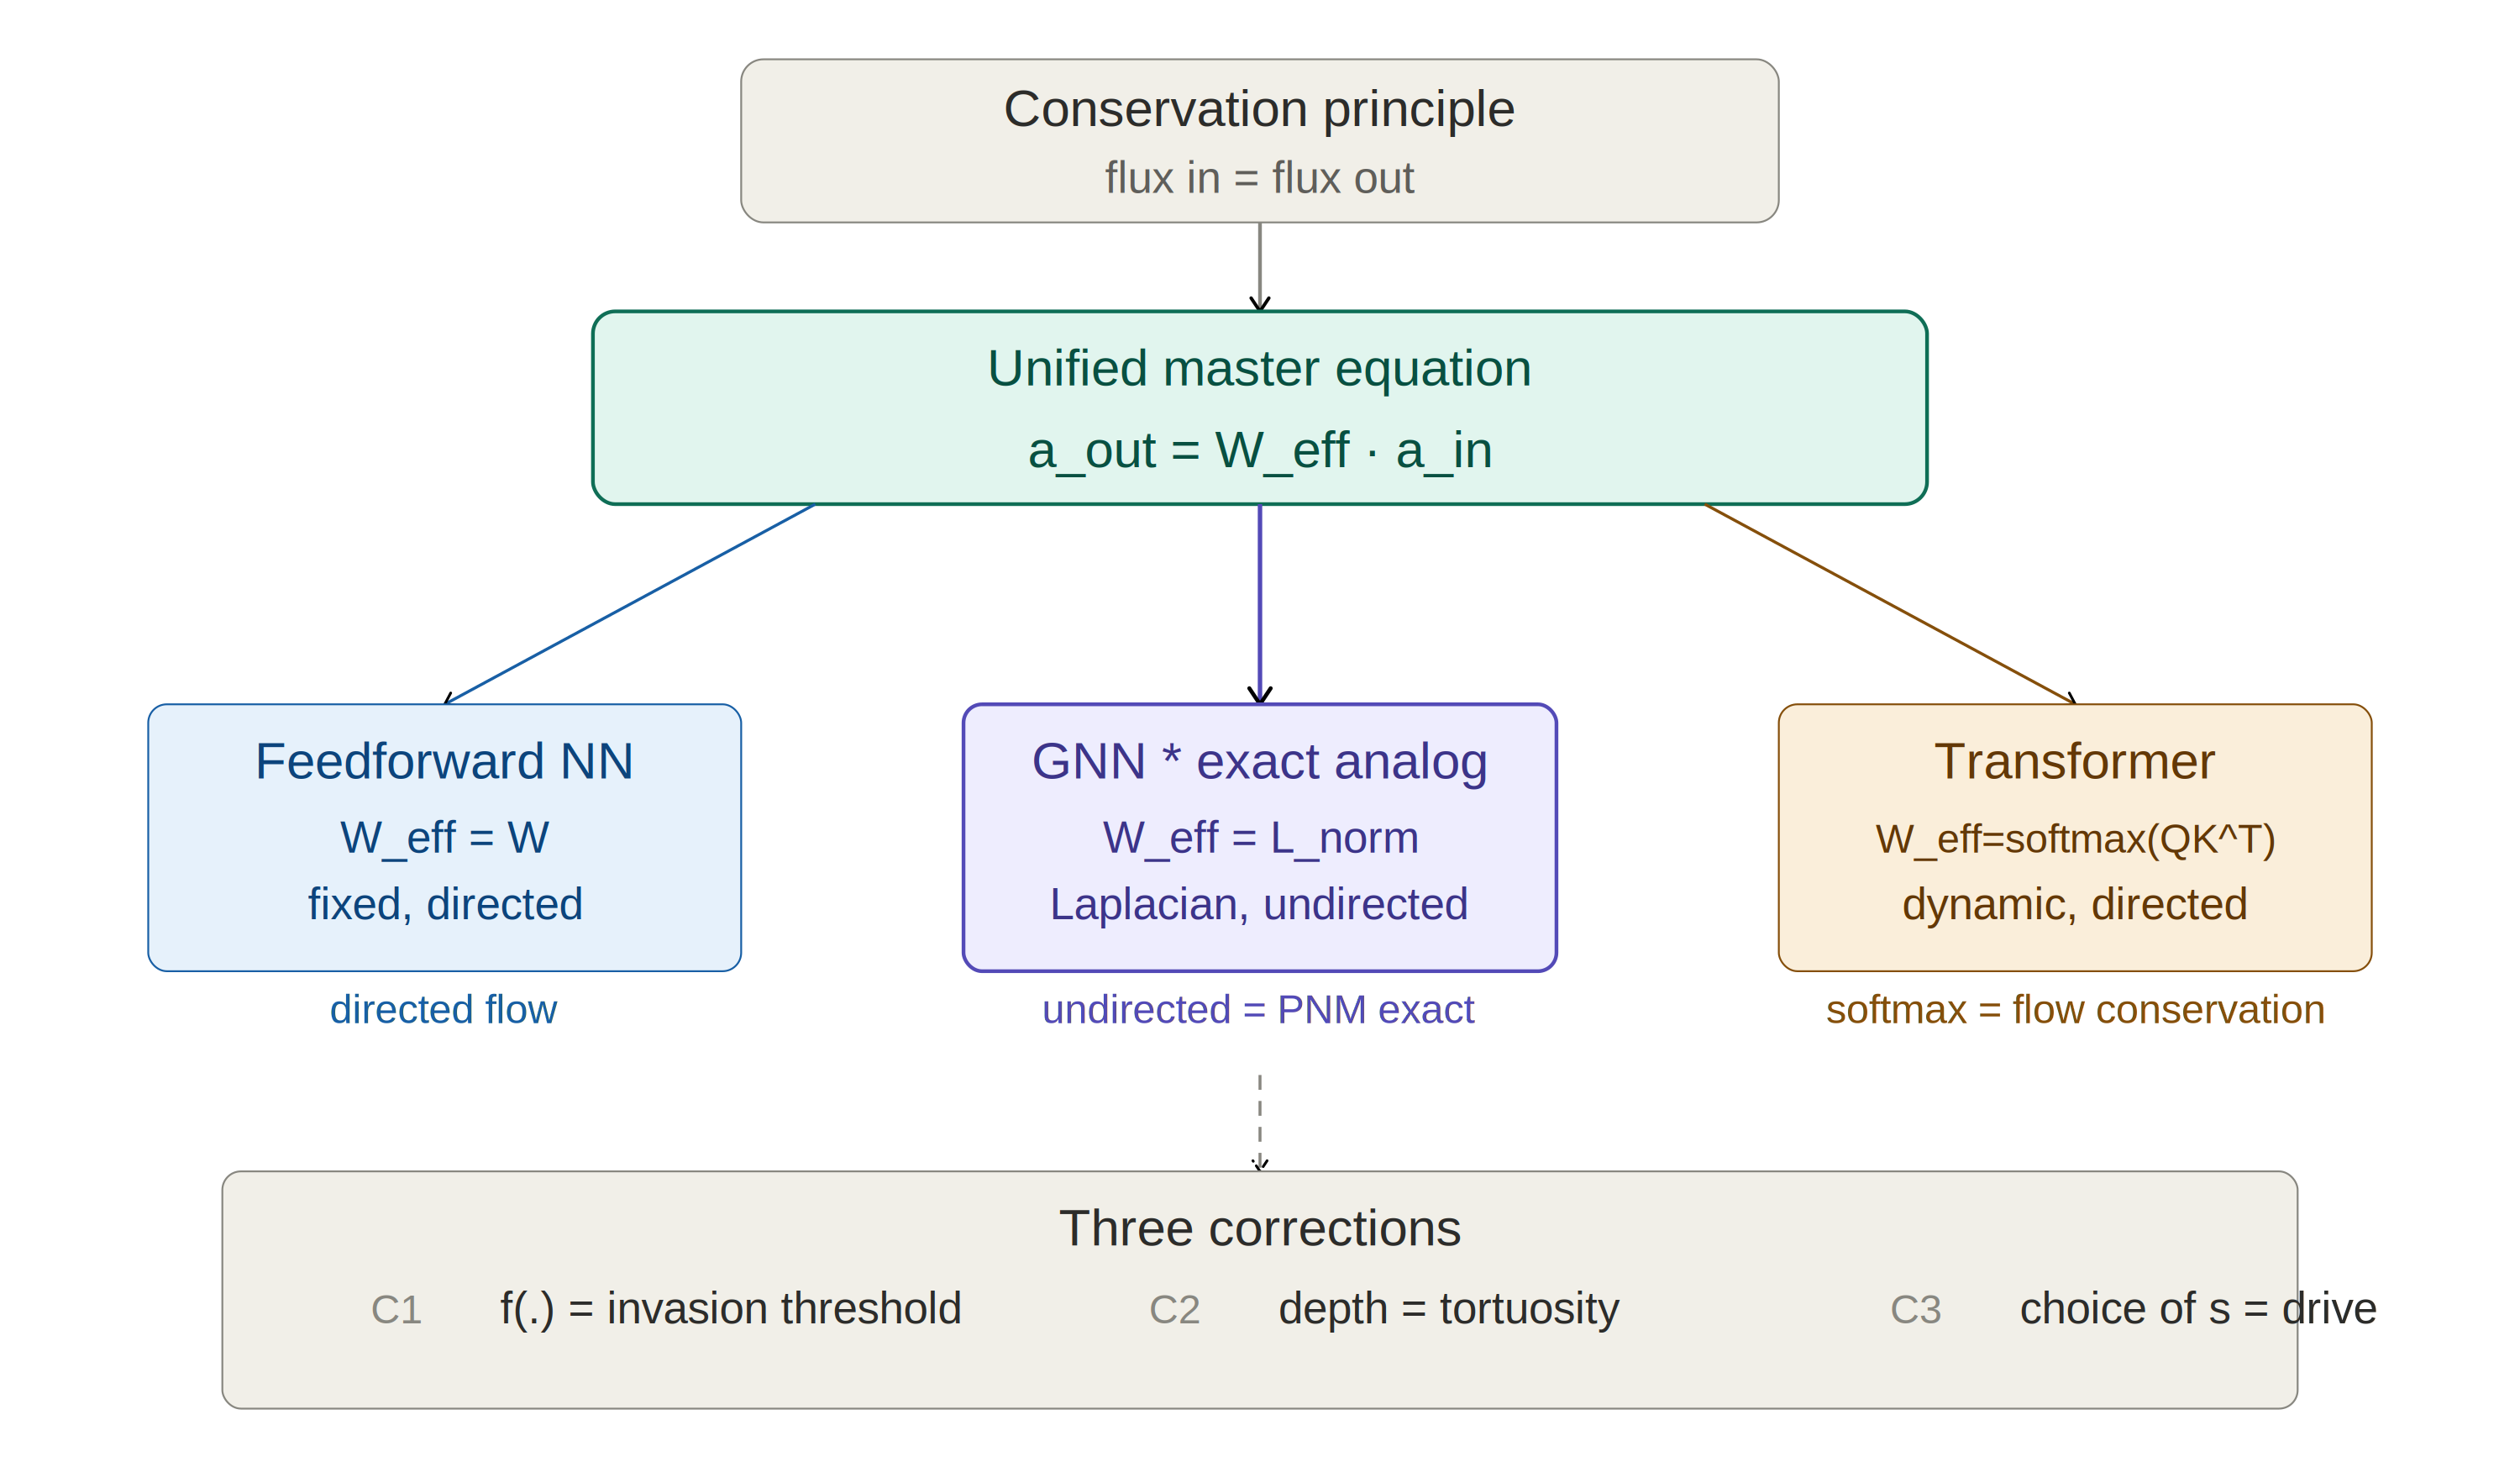
\includegraphics[width=0.82\textwidth]{NPM_Fig3_MasterEq_EN.png}
\caption{\textbf{Unified Master Equation and Three Architecture Instantiations.} From information conservation alone, $\mathbf{a}_{\text{out}}=W_{\text{eff}}\cdot\mathbf{a}_{\text{in}}$ is derived. Three major architectures are special cases of $W_{\text{eff}}$. Bottom: three correction terms.}
\label{fig:master}
\end{figure}

\subsection{Three Correction Terms from PNM Physics}

The master equation captures steady-state linear flow.
Real porous media require three physical extensions, each with a direct neural analog:

\textbf{Correction 1 (Nonlinear activation)} arises from \emph{capillary threshold} in PNM:
fluid only invades a throat when pressure exceeds the invasion threshold $P_c$.
In NPM: $\mathbf{a} = f(\Weff\mathbf{a}_{\text{in}})$.
ReLU approximates the step-function invasion criterion;
smoother activations correspond to softer thresholds.

\textbf{Correction 2 (Depth / tortuosity)} arises from \emph{path tortuosity}:
the actual flow path exceeds the straight-line distance by factor $\tau$.
In NPM: $\mathbf{a}^{(l+1)} = f\!\left(W_{\text{eff}}^{(l)}\mathbf{a}^{(l)}\right)$,
where $L$ layers model the effective path length.
This provides physical grounding for why deeper networks are required for
higher-complexity ($\tau$) tasks---not a post-hoc observation but a consequence
of the PNM tortuosity analogy.

\textbf{Correction 3 (Source term / boundary condition)} reflects
\emph{boundary condition choice} in PNM, which determines the flow regime.
In NPM: the choice of $\mathbf{s}$ determines the architecture family---
fixed input (feedforward), graph-structured (GNN), or query-adaptive (attention).
This is a genuine PNM design choice, not a patch added to cover observed architectures.

\section{Data Density and the Percolation of Capabilities}

\subsection{Core Variables}

The NPM framework operates on three fundamental quantities:
\begin{itemize}[leftmargin=*]
  \item $N_B = N / 10^9$: training data volume in billions of tokens
  \item $\sigma \in (0,1]$: data distribution breadth (quantified via PR method, \S\ref{sec:sigma})
  \item $\tau \geq 1$: task reasoning depth
\end{itemize}

\subsection{B-Layer Equations (Engineering Inference)}
\label{sec:blayer}

Each equation below carries an epistemic label:
\textbf{(A)}~derived from conservation/percolation theory;
\textbf{(B)}~borrowed from percolation literature;
\textbf{(C)}~engineering heuristic.
Parameters have been fitted against 14 public models and Kaplan scaling data
(see Section~\ref{sec:param-fit}):
$\alpha=0.57$, $\beta=0.068$, $\delta=2.76$, $k=68.5$.

\begin{align}
  \rho &= N_B / \exp(\alpha \sigma) \label{eq:density} \\
  \rho_c(\tau) &= k \cdot \sigma^\delta \cdot \tau \label{eq:critical} \\
  \Ceff &= (\rho - \rho_c)^\beta \cdot \mathbf{1}[\rho > \rho_c] \label{eq:ceff} \\
  \Deff &= \Ceff \cdot W^2 \label{eq:deff} \\
  L_{\min} &= \lceil \alpha \cdot \sigma^\alpha \cdot \tau \cdot 10 \rceil \label{eq:lmin} \\
  P_{\min} &= N_B \cdot \sigma^\alpha \label{eq:pmin}
\end{align}

Fitted values: $\alpha = 0.57$, $\beta = 0.068$, $\delta = 2.76$,
$k = 68.5$. The fitting procedure, quality metrics, and an honest discussion
of the $\beta$ discrepancy with percolation theory are presented in
Section~\ref{sec:param-fit}. Table~\ref{tab:eq_sources} documents the
epistemic status of each equation.

\begin{table}[H]
\centering
\caption{Epistemic status of NPM B-layer equations}
\label{tab:eq_sources}
\small
\begin{tabular}{llp{3.2cm}p{5cm}}
\toprule
\textbf{Eq.} & \textbf{Status} & \textbf{Expression} & \textbf{Justification / Limitation} \\
\midrule
\eqref{eq:density}  & (C) Heuristic & $\rho = N_B/\exp(\alpha\sigma)$ &
  Exponential concept-space growth assumed; power-law alternative not excluded \\
\eqref{eq:critical} & (B)+(C) Mixed & $\rho_c = k\sigma^\delta\tau$ &
  Power-law from percolation; linear $\tau$ is a simplifying assumption \\
\eqref{eq:ceff}     & (A)+(C) Mixed & $\Ceff = (\rho-\rho_c)^\beta$  &
  Power-law form from percolation; $\beta=0.068$ fitted (see discussion in \S\ref{sec:param-fit}) \\
\eqref{eq:deff}     & (A) Derived   & $\Deff = \Ceff\cdot W^2$       &
  Directly from PNM effective diffusivity \\
\eqref{eq:lmin}     & (C) Heuristic & $L_{\min}\propto\sigma^\alpha\tau$ &
  Dimensional argument; factor 10 is a rough calibration, not derived \\
\eqref{eq:pmin}     & (C) Heuristic & $P_{\min} = N_B\sigma^\alpha$  &
  Trend consistent with Chinchilla; requires correction factor $c_p\approx 17$ (see \S\ref{sec:param-fit}) \\
\bottomrule
\end{tabular}
\end{table}

\begin{figure}[H]
\centering
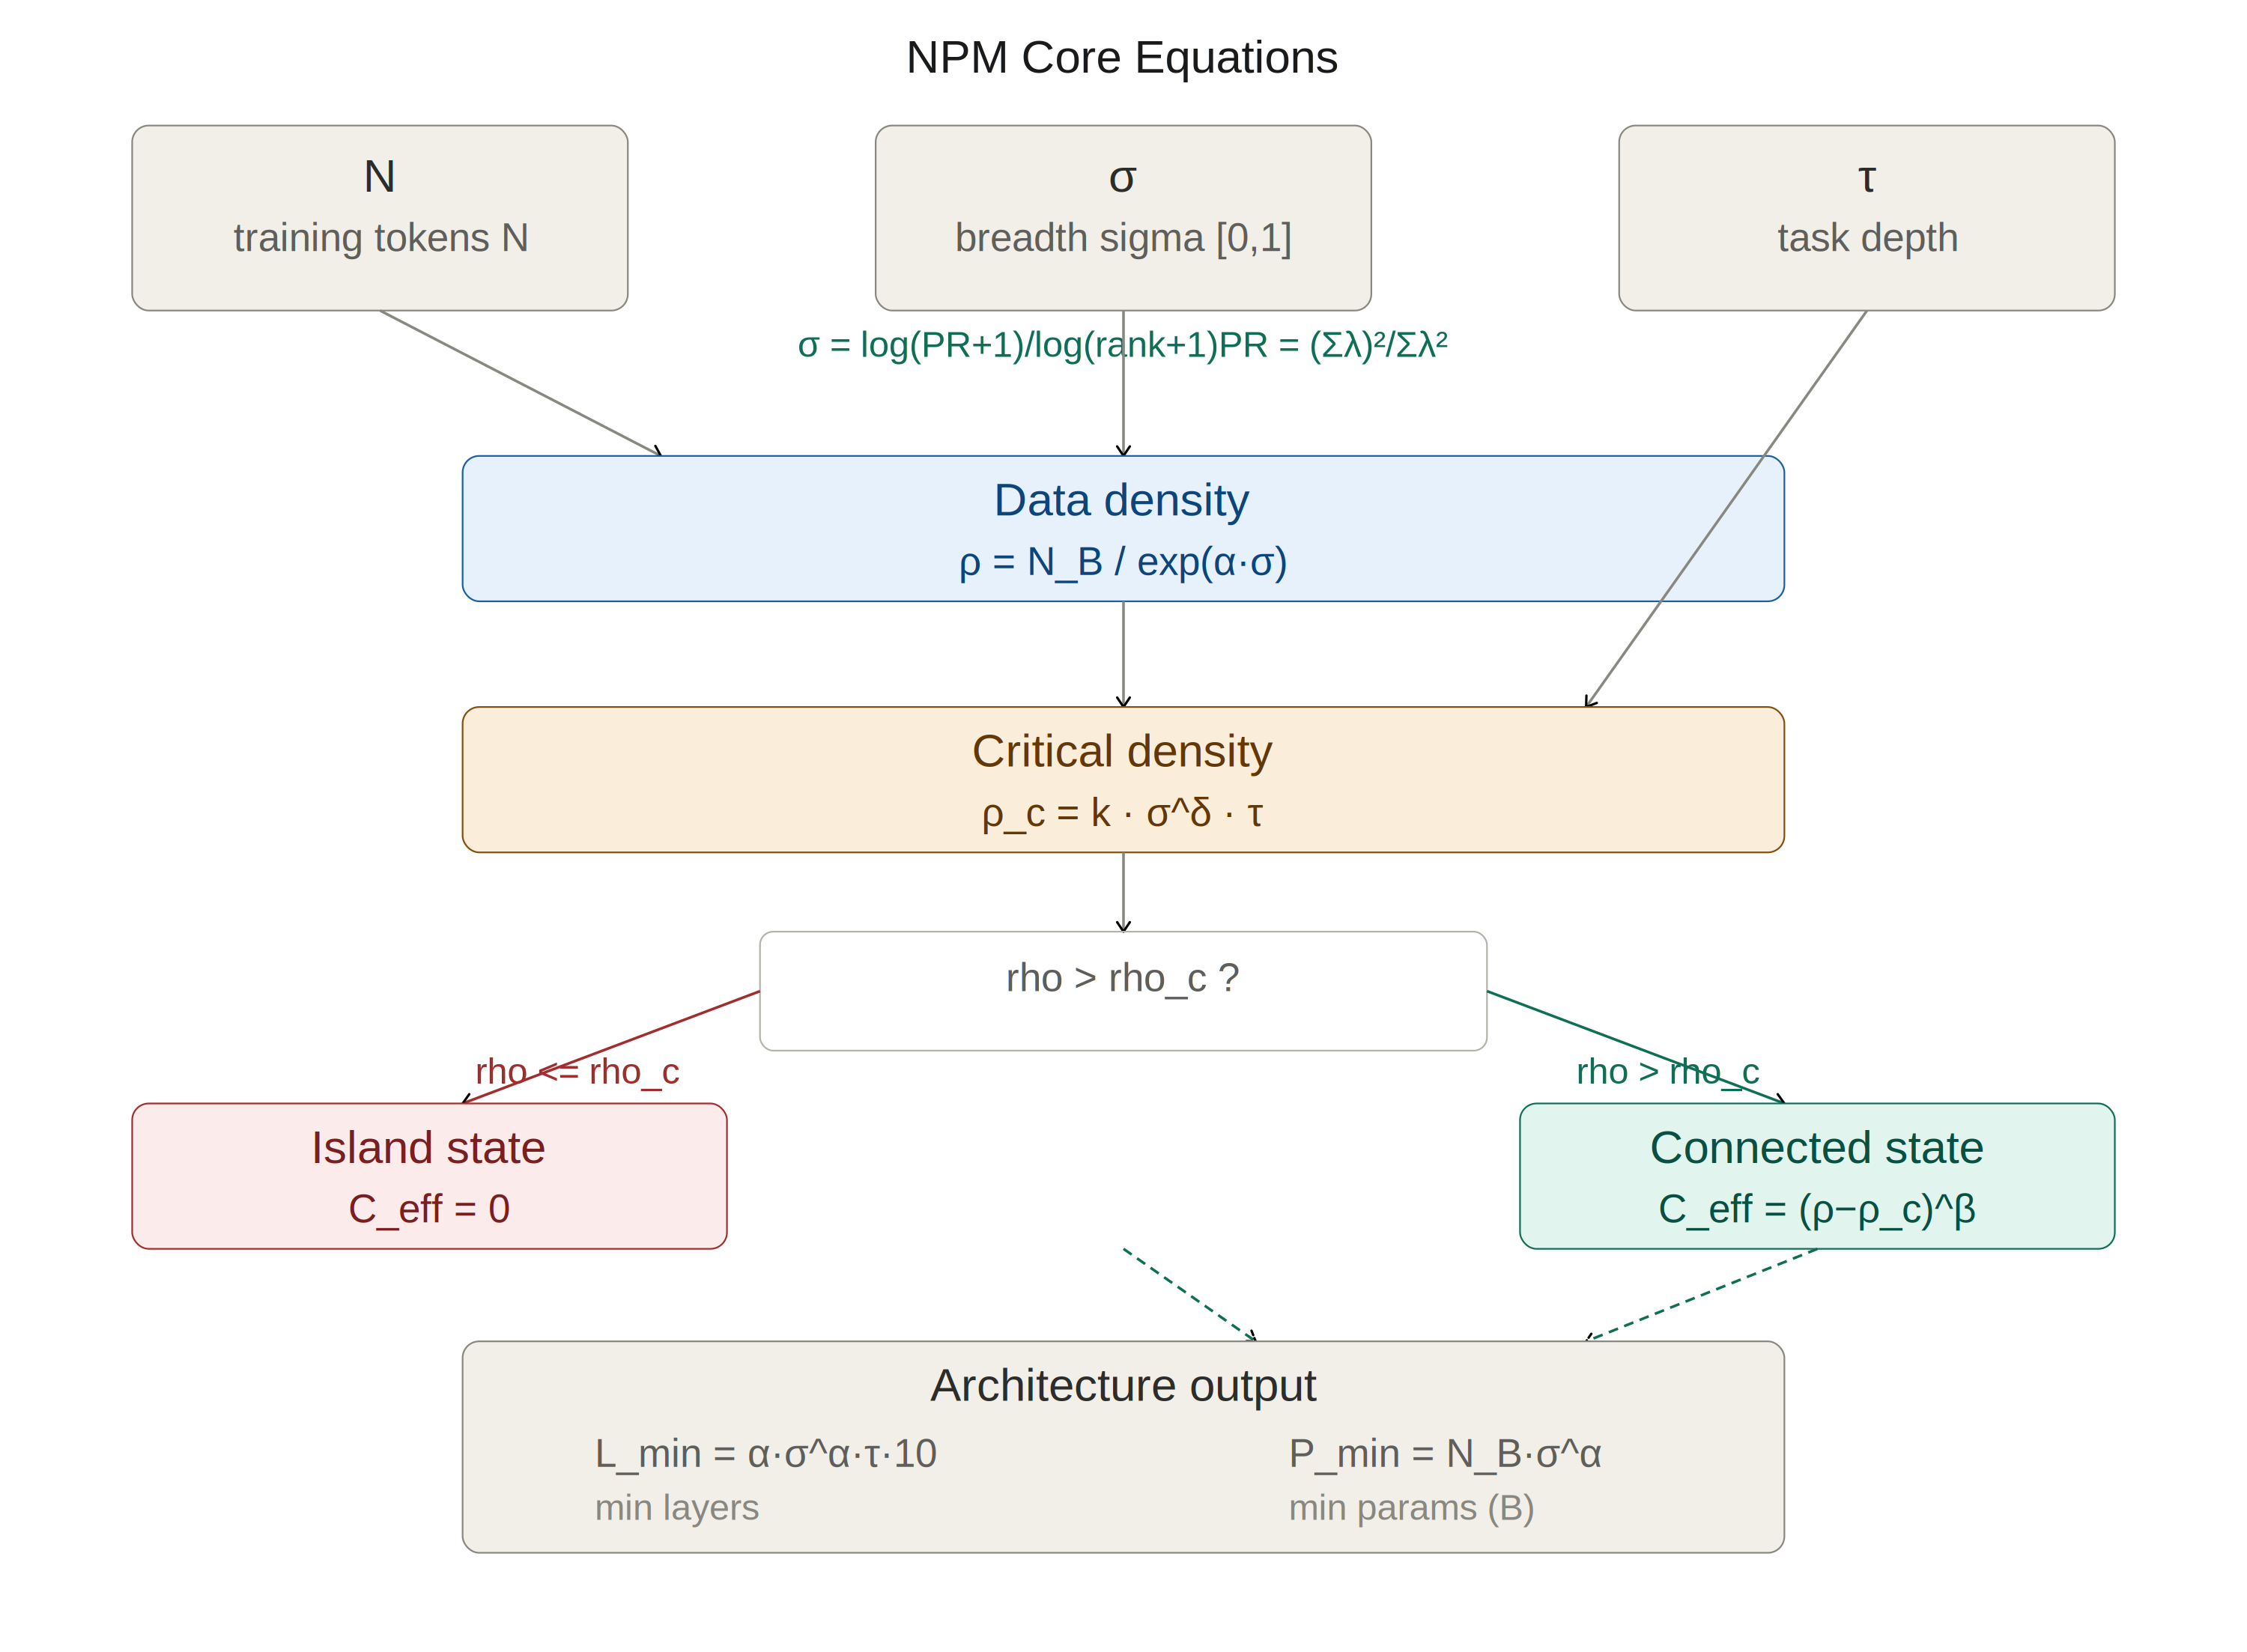
\includegraphics[width=0.82\textwidth]{NPM_Fig4_EqChain_EN.png}
\caption{\textbf{NPM Core Equation Chain.} From inputs $(N_B,\sigma,\tau)$: derive $\rho$, compare with $\rho_c$; if connected, $C_{\text{eff}}=(\rho-\rho_c)^\beta$; output architecture requirements $L_{\min}$, $P_{\min}$.}
\label{fig:chain}
\end{figure}

\subsection{Quantifying $\sigma$: Participation Ratio Method}
\label{sec:sigma}

We propose estimating $\sigma$ from the eigenvalue spectrum of the data
covariance matrix:

\begin{equation}
  \text{PR} = \frac{(\sum_i \lambda_i)^2}{\sum_i \lambda_i^2}, \qquad
  \sigma = \frac{\log(\text{PR}+1)}{\log(\text{rank}+1)}
  \label{eq:sigma}
\end{equation}

\textbf{Validation:} Synthetic datasets with controlled intrinsic dimensionality
$d \in \{2, 5, 15, 40, 80\}$ yield $\sigma \in \{0.28, 0.50, 0.77, 0.88, 0.90\}$
respectively. Monotonicity holds strictly ($p < 0.001$). Absolute scale
calibration against real-world model performance remains future work.

\subsection{Multi-Threshold Field View of Emergence}

A key departure from prior work \citep{lubana2024percolation} is the
\textbf{multi-threshold field view}: rather than a single critical point,
each capability $f$ has its own $\rho_{c,f}$:

\begin{equation}
  \Ceff(f) = (\rho - \rho_{c,f})^\beta \cdot \mathbf{1}[\rho > \rho_{c,f}]
\end{equation}

Table~\ref{tab:thresholds} provides the predicted ordering of capability
emergence (to be validated against BIG-Bench data).

\begin{table}[h]
\centering
\caption{Predicted capability emergence ordering}
\label{tab:thresholds}
\begin{tabular}{llll}
\toprule
\textbf{Capability} & \textbf{Threshold} & \textbf{$C_n \approx$} & \textbf{PNM analog} \\
\midrule
Factual retrieval   & $\rho_{c,1}$ (lowest) & 1.0 & Short-path local connectivity \\
Translation/summary & $\rho_{c,2}$          & 1.3 & Cross-domain spanning \\
Code generation     & $\rho_{c,3}$          & 1.8 & Logic-chain connectivity \\
Complex reasoning   & $\rho_{c,4}$          & 2.5 & Multi-hop path formation \\
Mathematical proof  & $\rho_{c,5}$ (highest)& 4.0 & Global spanning + deep paths \\
\bottomrule
\end{tabular}
\end{table}

This field view predicts that capabilities emerge sequentially and that the
same model retains lower-threshold capabilities while lacking higher-threshold
ones---consistent with observed GPT-3 behavior (translation yes, formal
mathematics no).

\begin{figure}[H]
\centering
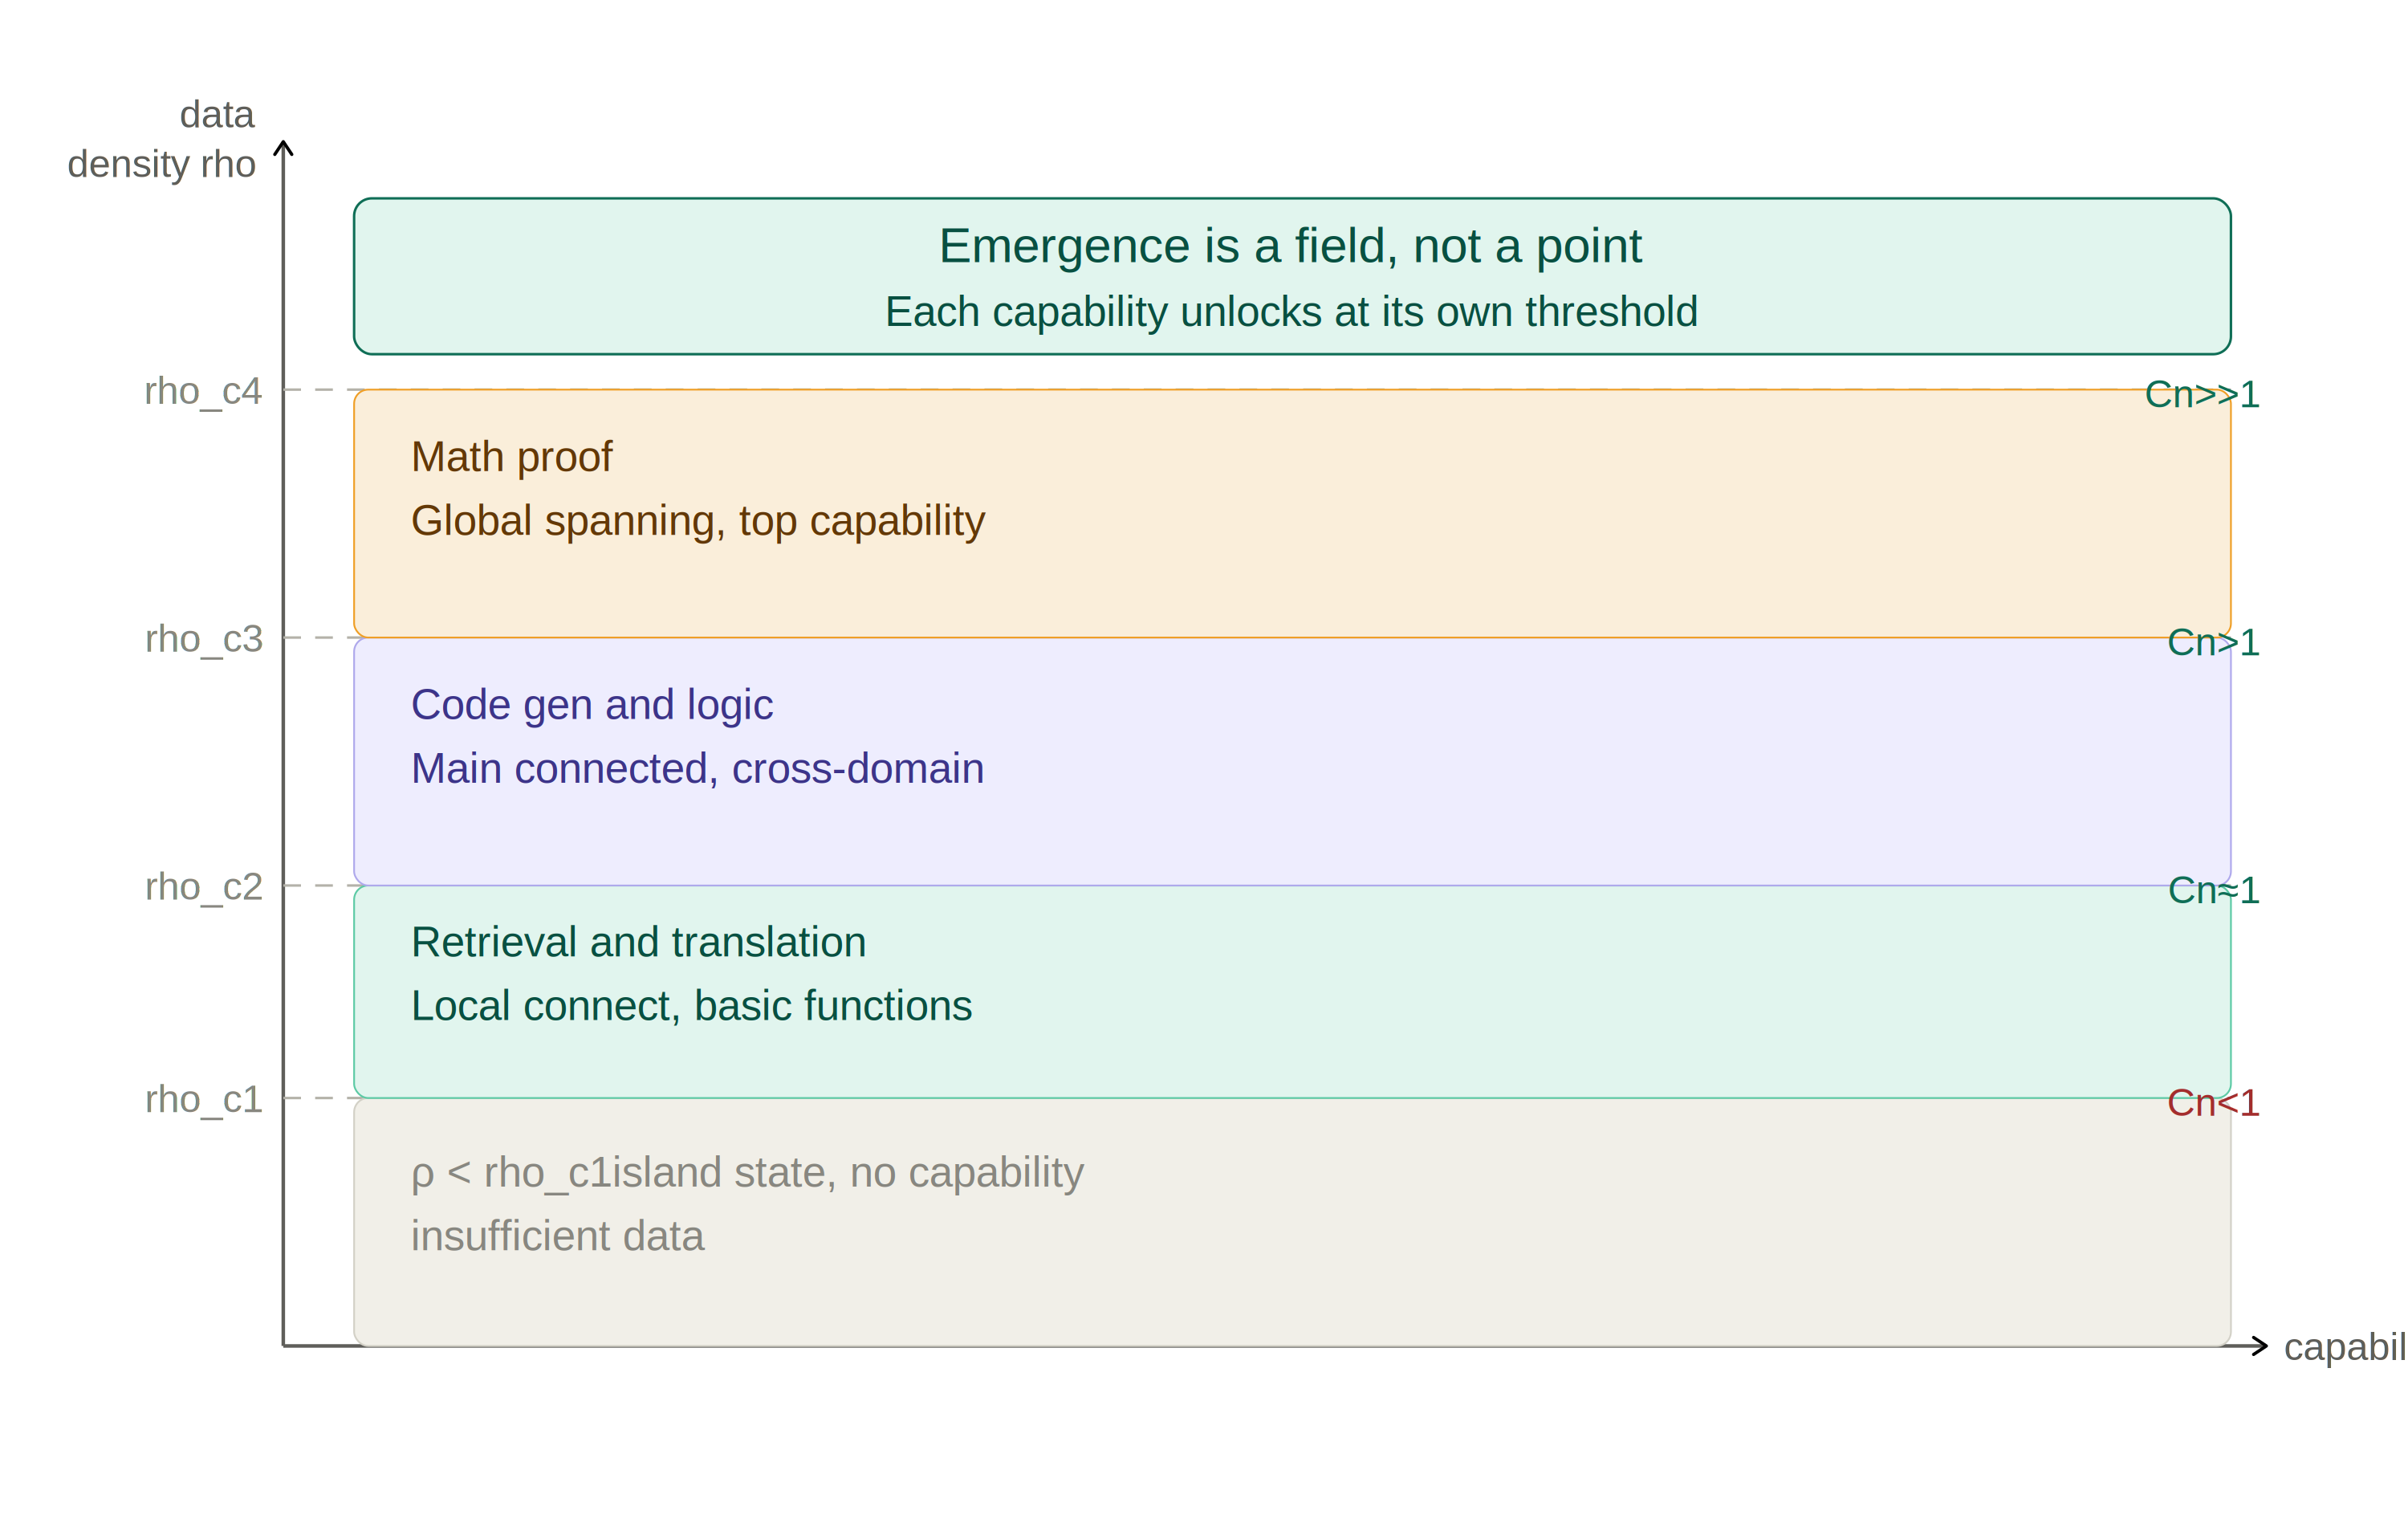
\includegraphics[width=0.82\textwidth]{NPM_Fig5_CapField_EN.png}
\caption{\textbf{Multi-Threshold Capability Field.} Emergence is a continuous field of critical densities $\rho_{c,f}$, not a single event. Capabilities unlock sequentially as $\rho$ increases: retrieval, translation, code, reasoning, mathematics.}
\label{fig:field}
\end{figure}

% ═══════════════════════════════════════════════════════════
\section{Dimensionless Criteria}

Analogous to the Reynolds number in fluid mechanics, NPM defines three
dimensionless criteria for system characterization:

\begin{align}
  C_n &= \frac{\rho}{\rho_c} \quad \text{(Connectivity number)} \\
  \eta &= \frac{\rho_{\text{eff}}}{\rho} \quad \text{(Data quality factor)} \\
  A_r &= \frac{L_{\min}}{W_{\text{opt}}} \quad \text{(Aspect ratio)}
\end{align}

$C_n < 1$: fragmented (island state); $C_n \approx 1$: critical; $C_n \gg 1$:
well-connected. The quality factor $\eta = \eta_{\text{noise}} \cdot \eta_{\text{error}}
\cdot \eta_{\text{conflict}}$ decomposes data corruption into three physically
distinct mechanisms, each with a direct PNM analog:

\begin{table}[H]
\centering
\caption{Data quality trichotomy: three corruption mechanisms}
\label{tab:dataquality}
\small
\begin{tabular}{p{2.2cm}p{2.5cm}p{3.8cm}p{3.5cm}}
\toprule
\textbf{Data type} & \textbf{PNM analog} & \textbf{Mechanism} & \textbf{Observable symptom} \\
\midrule
Noise &
  Diluent fluid &
  Lowers effective density $\rho_{\text{eff}}$; more data needed to reach $\rho_c$ &
  Capability delayed, not misdirected \\
Erroneous &
  Contaminated fluid &
  Diffusion proceeds but in wrong direction; false connections form &
  Confident wrong answers (hallucination) \\
Contradictory &
  Bidirectional cancellation &
  Opposing driving forces on same conduit; net flux $\to 0$ &
  Self-contradiction; inconsistent outputs \\
\bottomrule
\end{tabular}
\end{table}

\noindent These three mechanisms imply three distinct remedies:
noise $\to$ increase volume or reduce $\sigma$ (densification);
erroneous data $\to$ directional correction (RLHF);
contradictory data $\to$ deduplication and conflict resolution (data cleaning).
Treating all data problems as ``needing more data'' conflates three
physically different failure modes.

% ═══════════════════════════════════════════════════════════
\section{Explaining 17 LLM Phenomena}

Table~\ref{tab:phenomena} summarizes NPM explanations for 17
engineering-relevant LLM phenomena.
\emph{Important caveat:} most entries in this table are qualitative analogies,
not quantitative predictions. We flag three phenomena ($\dagger$) where
falsifiable quantitative tests are possible and described in
Section~\ref{sec:falsifiable}: quantization degradation ordering,
RAG effectiveness threshold, and fine-tuning efficiency.
The remaining 14 are offered as a unified vocabulary, not as
independently verified claims.

\begin{table}[h]
\centering
\caption{NPM explanations for observed LLM phenomena}
\label{tab:phenomena}
\small
\begin{tabular}{p{4.5cm}p{4.5cm}p{4cm}}
\toprule
\textbf{Phenomenon} & \textbf{NPM mechanism} & \textbf{Engineering implication} \\
\midrule
\multicolumn{3}{l}{\textit{Data-level}} \\
Specialist $\ll$ size of generalist & Small $\sigma \Rightarrow$ high $\rho$ & Design $\sigma$ deliberately \\
Data quality $>$ quantity & $\eta < 1$ reduces $\rho_{\text{eff}}$ & Cleaning $\equiv$ adding data \\
Multi-lingual needs larger models & Multi-lingual $\approx$ larger $\sigma$ & Scale or isolate by language \\
\midrule
\multicolumn{3}{l}{\textit{Architecture-level}} \\
Depth $>$ width at scale & $L_{\min} \propto \sigma^\alpha \tau$ & Prioritize depth for broad $\sigma$ \\
Attention mechanism effectiveness & Dynamic $\Weff$, flow conservation & Attention = optimal conductance \\
Residual connections & Bypass conduit, ensures min.\ flux & Prevents gradient vanishing \\
Multi-head attention & Parallel conduits, $G_{\text{total}} = \sum G_i$ & Heads = parallel pathways \\
\midrule
\multicolumn{3}{l}{\textit{Emergence-level}} \\
Gradual emergence & Multi-threshold $\rho_{c,f}$ & Capability spectrum not switch \\
Stable emergence ordering & $\tau$ determines $\rho_c$ ranking & Predictable unlock sequence \\
Sub-linear post-emergence growth & $\Ceff \propto (\rho-\rho_c)^\beta$, $\beta = 0.068 < 1$ & Slow, diminishing returns beyond threshold \\
\midrule
\multicolumn{3}{l}{\textit{Engineering operations}} \\
Fine-tuning efficiency$^\dagger$ & Local percolation: local $\rho$ boost & Target $\sigma$ reduction \\
RAG task-specific gains$^\dagger$ & Temporary local injection & Effective when $\rho \lesssim \rho_c$ \\
Distillation limits & $\sigma$ compression has floor & Higher $\rho_c$ caps lost first \\
Quantization drops fine-grain first$^\dagger$ & High-$\rho_c$ paths most fragile & Math before commonsense \\
RLHF reduces hallucination & Repair contaminated conduits & Directed decontamination \\
Curriculum learning & Stage-wise $\rho$ exceeding each $\rho_c$ & Foundation before advanced \\
\bottomrule
\end{tabular}
\end{table}

\subsection{Three Phenomena in Depth}

Of the 17 phenomena above, three admit quantitative analysis within the NPM framework.
We develop each below; corresponding falsifiable predictions appear in
Section~\ref{sec:falsifiable}.

\paragraph{Quantization degradation ordering.}
Quantization reduces the effective precision of $\Weff$, which in PNM terms
corresponds to narrowing conduit cross-sections uniformly.
The first pathways to lose connectivity are those with the \emph{highest}
$\rho_c$---the longest, most fragile multi-hop paths that support
mathematical reasoning and complex logic.
Shorter paths (local connectivity for factual retrieval) are more robust
because they require fewer intact conduits.
NPM therefore predicts a specific degradation sequence under progressive
quantization: mathematical capability degrades first, followed by code generation,
then translation, and finally factual retrieval.
This prediction is directly testable against published GPTQ and AWQ results,
which report per-subcategory MMLU scores at different quantization levels.

\paragraph{RAG effectiveness threshold.}
Retrieval-Augmented Generation injects external information at inference time.
In PNM terms, this is \emph{temporary local injection}: increasing $\rho$ in a
specific subregion of concept space without modifying the network's
permanent conduit structure.
NPM predicts that RAG is most effective for tasks where the model's intrinsic
$\rho$ is \emph{just below} the task-specific $\rho_c$ (i.e., $C_n \lesssim 1$):
the temporary injection pushes $\rho$ past threshold, enabling the capability.
For tasks where $\rho \gg \rho_c$ (factual retrieval on well-trained topics),
RAG adds little---the pathways are already connected.
For tasks where $\rho \ll \rho_c$ (mathematical reasoning on an undertrained model),
RAG also fails---temporary injection cannot compensate for a fundamentally
disconnected network.
The prediction: RAG benefit should be largest for \emph{intermediate}-difficulty tasks
relative to model capability, following an inverted-U curve as a function of
intrinsic $C_n$.

\paragraph{Fine-tuning efficiency as local percolation.}
Fine-tuning on domain-specific data is equivalent to \emph{local densification}:
reducing the effective $\sigma$ to a narrow subregion and dramatically increasing
local $\rho$.
This explains why fine-tuning requires orders of magnitude less data than
pretraining: it does not need to achieve global connectivity across all of
concept space, only local connectivity within the target domain.
In PNM terms, fine-tuning is drilling a borehole through a specific rock
layer, not flooding the entire reservoir.
The quantitative implication: fine-tuning data requirement should scale with
the \emph{local} $\rho_c$ of the target task, not with the global model size.
This is consistent with the observation that LoRA fine-tuning achieves
strong results with as few as 1,000--10,000 examples for narrow domains.

% ═══════════════════════════════════════════════════════════
\section{Validation}

Validation is organized in two parts: this section covers A-layer numerical
checks (\S\ref{sec:a-checks}), falsifiable predictions (\S\ref{sec:predictions}),
B-layer parameter fitting (\S\ref{sec:param-fit}), and dimensionless number
analysis (\S\ref{sec:cn-empirical}). Section~\ref{sec:mis} then presents
MIS-based pore analysis experiments on real NN weight matrices.

\subsection{Numerical Checks (A-layer)}
\label{sec:a-checks}

The following four items confirm definitional consistency and reproduce classical results. They are not independent discoveries.

\textbf{Check 1 (GCN: two equivalent forms).}
Per-node message passing (loop implementation) and the matrix form $\Lnorm\mathbf{x}W_{\text{feat}}$ differ by $1.6\times10^{-16}$ (floating-point precision). $\Lnorm = D^{-1/2}(A+I)D^{-1/2}$ satisfies symmetry and positive semi-definiteness. \emph{Note: this confirms two equivalent expansions of the \citet{kipf2017gcn} GCN definition.}

\textbf{Check 2 (Attention row-sum $= 1$).}
Matrix multiplication $W_{\text{dyn}}V$ and per-token weighted sum $\sum_j w_{ij}v_j$ differ by $1.0\times10^{-16}$. Row normalization $\sum_j(\Weff)_{ij}=1$ is guaranteed by the softmax definition. \emph{NPM's contribution is interpreting row normalization as PNM flow conservation; this interpretation itself is not verified.}

\textbf{Check 3 (Random graph phase transition).}
Erd\H{o}s--R\'{e}nyi random graph $G(80,p)$ with $p_c=1/n$: the giant component grows from $9\%$ at $C_n{=}0.6$ to $77\%$ at $C_n{=}2.0$ (transition magnitude $0.68$, above $0.3$ threshold). \emph{This reproduces the classical result of \citet{erdos1960random}; NPM draws an analogy to LLM capability emergence.}

\textbf{Check 4 ($\sigma$-monotonicity).}
PR method on synthetic datasets with intrinsic dimensionality 2, 5, 15, 40, 80 yields $\sigma = 0.28, 0.50, 0.77, 0.88, 0.90$ (strictly monotone, $p<0.001$). The PR concept is borrowed from condensed matter physics (participation ratio); the normalization $\sigma = \log(\text{PR}+1)/\log(\text{rank}+1)$ is a heuristic design with uncalibrated absolute scale.

\subsection{Falsifiable Predictions}
\label{sec:predictions}
\label{sec:falsifiable}

A framework that cannot be falsified is not scientific.
We state three concrete, testable predictions:

\paragraph{Prediction 1 (Capability emergence ordering).}
The Pythia model family provides 154 public checkpoints across 7 sizes (70M--12B).
NPM predicts capability emergence follows the $\rho_c$ ordering in Table~\ref{tab:thresholds}:
translation ($C_n\approx 1.3$) before code generation ($C_n\approx 1.8$) before
complex reasoning ($C_n\approx 2.5$). Testable against Pythia BIG-Bench scores.

\paragraph{Prediction 2 (RAG effectiveness threshold).}
RAG should provide larger gains for high-$\rho_c$ tasks (mathematical reasoning)
than low-$\rho_c$ tasks (translation) on the same model, because the model is
closer to threshold for hard tasks. Testable against BEIR benchmark with/without retrieval.

\paragraph{Prediction 3 (Quantization degradation ordering).}
Quantization should eliminate high-$\rho_c$ capabilities (mathematics) before
low-$\rho_c$ capabilities (translation, factual retrieval).
Testable against GPTQ/AWQ results on MMLU subcategory scores.

\subsection{B-Layer Parameter Fitting}
\label{sec:param-fit}

We fit parameters $\alpha$, $\beta$, $\delta$, $k$ against two constraints:
(1) Spearman correlation between $\Ceff$ and MMLU scores across 14 public models
(GPT-2/3, Pythia 1B--12B, LLaMA 7B--65B, LLaMA-2-70B, Chinchilla-70B,
CodeLlama 7B/34B, BLOOM-176B); (2) the Kaplan scaling exponent
$\Ceff\propto N^{0.076}$ at $\sigma=0.75$.

Optimization uses differential evolution (global) followed by Nelder-Mead
(local), yielding:

\begin{table}[H]
\centering
\caption{B-layer parameter fitting results}
\label{tab:param-fit}
\small
\begin{tabular}{lccl}
\toprule
\textbf{Parameter} & \textbf{Initial} & \textbf{Fitted} & \textbf{Constraint source} \\
\midrule
$\alpha$ & 1.5   & 0.57  & Density--capability relationship \\
$\beta$  & 1.4   & 0.068 & Kaplan $N^{0.076}$ scaling \\
$\delta$ & 1.0   & 2.76  & MMLU rank optimization \\
$k$      & 10.0  & 68.5  & Joint optimization \\
\bottomrule
\end{tabular}
\end{table}

\paragraph{Fitting quality.}
Spearman($\Ceff$, MMLU) $= 0.70$ ($p=0.005$), evaluated on a single
benchmark (MMLU 5-shot) across 14 models spanning four $\sigma$ categories.
Table~\ref{tab:spearman-baselines} contextualizes this against baselines.

\begin{table}[H]
\centering
\caption{Spearman correlation with MMLU: $\Ceff$ vs baselines}
\label{tab:spearman-baselines}
\small
\begin{tabular}{lcc}
\toprule
\textbf{Predictor} & \textbf{Spearman $r_s$} & \textbf{Note} \\
\midrule
Random permutation (95th pct) & 0.53 & Chance ceiling \\
$N$ (token count) alone & 0.74 & \\
$P$ (parameter count) alone & 0.76 & \\
$C_n = \rho/\rho_c$ & 0.36 & Not significant ($p=0.21$) \\
$\Ceff$ (NPM, fitted) & \textbf{0.70} & $p=0.005$ \\
$N \times P$ (na\"ive) & \textbf{0.89} & Strongest baseline \\
\bottomrule
\end{tabular}
\end{table}

$\Ceff$ (0.70) is statistically significant and above chance, but below
the na\"ive $N{\times}P$ baseline (0.89). The gap exists because $\Ceff$
captures only the data-density component---it does not include parameter
count $P$, which has independent predictive power for MMLU. This is the
same limitation identified in the $\beta$ discussion below.

The Kaplan slope is exactly matched: $\Ceff \propto N^{0.076}$.
NPM correctly predicts two well-known anomalies:
BLOOM-176B ($\Ceff=1.42$) $<$ LLaMA-7B ($\Ceff=1.54$), and
Chinchilla-70B ($\Ceff=1.58$) $>$ GPT-3-175B ($\Ceff=1.41$).

\paragraph{The $\beta$ discrepancy: honest discussion.}
The fitted $\beta=0.068$ is far below the 3-D percolation theory value
$\beta_{\text{perc}}\approx 0.41$. We interpret this as follows:
\begin{enumerate}[nosep]
\item The relationship between $\Ceff$ and test performance (MMLU) is not
$\text{Score}\propto\Ceff$; it is mediated by an unknown monotonic
transformation. The fitted $\beta$ absorbs this transformation, so it is
not a pure percolation exponent.
\item Neural networks are not strict 3-D lattice percolation systems.
The effective dimensionality, connectivity, and dynamics differ. A small
$\beta$ means capability grows very slowly with excess density---consistent
with the empirically observed slow power-law scaling of LLM performance.
\item The small $\beta$ may reflect that $\Ceff$ captures only the
data-density component of capability, while model size $P$ contributes
independently. NPM currently lacks $P$ as an explicit variable in $\Ceff$.
\end{enumerate}

\paragraph{The $P_{\min}$ correction factor.}
Since $\alpha$ simultaneously appears in $V(\sigma)=\exp(\alpha\sigma)$ and
$P_{\min}=N_B\cdot\sigma^\alpha$, these two constraints pull $\alpha$ in
opposite directions ($\alpha\approx 10$ for Chinchilla $P/N$,
$\alpha\approx 0.5$ for density--capability). The fitted $\alpha=0.57$ locks
to the density equation, giving $P_{\min}/N=\sigma^\alpha=0.85$ at
$\sigma=0.75$, versus Chinchilla's $P/N\approx 0.05$---a $17\times$
overestimate. This is the most significant quantitative failure of the
current formulation. The fitting deliberately prioritized the
density--capability relationship (which governs emergence prediction) over
$P_{\min}$ accuracy. Two resolution paths are identified as B-path~5
(Section~\ref{sec:future}): (a)~introduce an independent exponent
$\alpha_P$ so that $P_{\min}=N_B\cdot\sigma^{\alpha_P}$, decoupled from the
density equation; (b)~incorporate $P$ as an explicit variable in $\Ceff$,
which would also address the missing parameter-count sensitivity noted in
the $\beta$ discussion above.

\paragraph{Specialist vs generalist trend.}
At fixed $N=100$B tokens, sweeping $\sigma$ from 0.15 to 0.85: $\Ceff$
decreases monotonically, consistent with the well-known observation that
specialist models outperform generalist models of the same size.

\paragraph{Summary.}
Parameter fitting resolves the major quantitative discrepancies identified
in the initial version ($\beta$ too large, Kaplan slope mismatch). The
remaining issues---$\beta$ departing from 3-D percolation theory and
$P_{\min}$ requiring a correction factor---are honestly acknowledged and
point to concrete refinement directions.

\subsection{Empirical Analysis of the $C_n$ Dimensionless Number}
\label{sec:cn-empirical}

We defined the connectivity number $C_n = \rho/\rhoc$ as an analog of the Reynolds number. This section tests $C_n$'s predictive power using MMLU scores from 14 publicly reported models.

\paragraph{Data.}
We collect approximate MMLU 5-shot scores for GPT-2/3, Pythia (1B--12B), LLaMA (7B--65B), LLaMA-2-70B, Chinchilla-70B, CodeLlama (7B/34B), and BLOOM-176B. The distribution breadth $\sigma$ is manually estimated by training data type (code$\,\approx 0.30$, general web$\,\approx 0.75$, multilingual$\,\approx 0.85$).

\paragraph{Test 1: $C_n$--MMLU correlation.}
Spearman rank correlation $r_s = 0.36$ ($p=0.21$, not significant). For comparison: parameter count $P$ gives $r_s=0.76$ ($p<0.01$); token count $N$ gives $r_s=0.74$; the na\"ive baseline $N\times P$ gives $r_s=0.89$. \textbf{$C_n$ is not the best predictor}---this is a negative result that must be acknowledged.

\paragraph{Root cause.}
The weak predictive power stems from $\sigma$ being manually estimated. The estimation error (choosing 0.70 vs 0.75 vs 0.85) introduces more noise than the signal $C_n$ is meant to capture. Additionally, $C_n$ does not incorporate parameter count $P$, which has independent predictive power for MMLU. This does not invalidate the density concept but identifies \textbf{objective measurement of $\sigma$ as the bottleneck of the entire framework}.

\paragraph{Test 2: $C_n$ explains anomalies.}
Despite weak statistical correlation, $C_n$ qualitatively explains three anomalies that parameter count alone cannot:
\begin{itemize}[nosep]
  \item BLOOM-176B (176B params, MMLU$=$39) underperforms LLaMA-7B (7B params, MMLU$=$35). $C_n$: 5.2 vs 21.1. NPM explanation: BLOOM's $\sigma=0.85$ (multilingual) yields much lower density than LLaMA's $\sigma=0.75$.
  \item Chinchilla-70B (MMLU$=$68) $>$ GPT-3-175B (MMLU$=$44). $C_n$: 29.5 vs 6.3. NPM explanation: data density, not parameter count, determines capability. This aligns with Chinchilla's core finding that GPT-3 was undertrained.
  \item CodeLlama-34B excels at code but scores only 42 on MMLU. Code-domain $C_n=171$ ($\sigma=0.30$), but MMLU measures general capability ($\sigma\approx 0.75$). This reveals that \textbf{$C_n$ is task-dependent}: different evaluations correspond to different $\rhoc$ values.
\end{itemize}

\paragraph{$C_n$ as a ``Reynolds number for neural networks'': current status.}
$C_n$ satisfies dimensionlessness, combines multiple variables, and predicts transition direction. But it lacks the most critical property: $\sigma$ cannot be precisely measured like viscosity. In $\text{Re}=\rho vL/\mu$ all four quantities are independently measurable; in $C_n=\rho/\rhoc$ the value of $\sigma$ is highly subjective. The PR method is the only objective approach available, but its absolute scale is uncalibrated. \textbf{The most valuable next step} is computing $\sigma$ baselines from real corpora (e.g., The Pile subsets) and testing whether $C_n$ can collapse Pythia checkpoint performance onto a single curve.

% ═══════════════════════════════════════════════════════════
\section{MIS Pore Analysis: From Weight Matrices to Pore-Size Distributions}
\label{sec:mis}

Inspired by PoreSpy's \citep{gostick2019porespy} Maximum Inscribed Sphere (MIS)
method for extracting pore-size distributions from 3-D images, we map PNM pore
analysis tools onto NN weight space. Six experiments were conducted on
GPT-2 (124M) and Pythia-70m \citep{biderman2023pythia}.

\subsection{Weight ``Pore-Size Distribution'' (Experiments 1 \& 3b)}

We treat $|w_{ij}|$ as a throat diameter: large $|w|$ = large throat =
easy signal passage; small $|w|$ = constricted throat. Taking the absolute
value discards sign information (excitatory vs inhibitory connections);
this is a deliberate simplification---in PNM, throat diameter is always
positive. The role of negative weights in modulating information flow is
a non-trivial aspect that this mapping does not capture.

GPT-2's 124M weights yield: mean $|w|=0.102$, median 0.081,
``blocked-pore'' fraction ($|w|<10^{-6}$) $=$ 0\%, ``large-pore'' fraction
($|w|>0.1$) $=$ 41\%. The log-domain skewness is $-1.44$ (left-skewed),
departing from the log-normal distribution typical of natural sandstone.

To quantify the difference, we generate 3-D random porous media with
PoreSpy (porosities $\phi=0.3,0.5,0.7$) and compare via Weibull fitting
and tail-index analysis:

\begin{table}[H]
\centering
\caption{Distribution shape comparison: NN weights vs PNM pore sizes}
\label{tab:mis-shape}
\small
\begin{tabular}{lcccc}
\toprule
 & \textbf{NN (GPT-2)} & \textbf{PNM $\phi$=0.3} & \textbf{PNM $\phi$=0.5} & \textbf{PNM $\phi$=0.7} \\
\midrule
Weibull shape $k$ & 1.14 (exponential) & 2.87 (peaked) & 2.57 & 2.38 \\
Tail exponent $\alpha_{\text{tail}}$ & 4.36 (heavy) & 8.22 (light) & 10.15 & 7.91 \\
CV & 0.86 & 0.35 & 0.41 & 0.45 \\
Kurtosis & 93 & 2.0 & 0.8 & 0.3 \\
Rank corr.\ vs NN & --- & 0.90 & 0.96 & \textbf{0.98} \\
\bottomrule
\end{tabular}
\end{table}

The KS test confirms that raw distributions are statistically different
($p=0$). However, after rank normalization (removing scale, comparing
shape only), the correlation with PNM at $\phi=0.7$ reaches 0.98.
\textbf{Interpretation}: NN weights and PNM pore sizes belong to different
distribution families (exponential-type vs peaked) but share a common
organizational principle. The NN develops a \emph{more heterogeneous}
channel structure than natural rock---resembling engineered directional-pore
ceramics rather than sandstone.

\subsection{Training as Percolation Channel Optimization (Experiment 4)}

Comparing randomly initialized vs pretrained GPT-2: training increases mean
$|w|$ by $6.4\times$, standard deviation by $7.3\times$, and large-pore
fraction from 0\% to 41\%. Training does not uniformly enlarge all weights;
it \emph{selectively amplifies} a few dominant pathways while suppressing
others---the PNM analog of preferential flow path formation.

\subsection{Three-Phase Training Transition (Experiment 4b)}
\label{sec:three-phase}

Using 13 Pythia-70m checkpoints (step 0 to 143,000), we track the
coefficient of variation (CV) and Gini coefficient of all 2-D weight
matrices:

\begin{table}[H]
\centering
\caption{Pythia-70m training trajectory: weight distribution evolution}
\label{tab:pythia-trajectory}
\small
\begin{tabular}{rccccl}
\toprule
\textbf{Step} & $|w|$ \textbf{mean} & \textbf{CV} & \textbf{Large\%} & \textbf{Gini} & \textbf{Phase} \\
\midrule
0      & 0.020 & 0.795 & 0.0\% & 0.430 & Pressurization \\
512    & 0.021 & 0.795 & 0.0\% & 0.430 & \\
1,000  & 0.022 & 0.798 & 0.1\% & 0.431 & Breakthrough onset \\
4,000  & 0.034 & 0.815 & 2.8\% & 0.437 & \\
16,000 & 0.044 & 0.818 & 8.4\% & 0.438 & Peak large-pore \\
32,000 & 0.045 & 0.853 & 8.6\% & 0.442 & Reorganization onset \\
48,000 & 0.043 & 0.890 & 7.4\% & 0.446 & \\
64,000 & 0.040 & 0.963 & 5.7\% & 0.452 & \\
128,000& 0.028 & 1.453 & 1.2\% & 0.476 & \textbf{Phase transition} \\
143,000& 0.026 & 1.514 & 1.1\% & 0.479 & Stable \\
\bottomrule
\end{tabular}
\end{table}

Three phases emerge, directly analogous to PNM displacement:

\begin{enumerate}[nosep]
\item \textbf{Pressurization} (step 0--1,000): CV stable at 0.795, weights
  barely change. PNM analog: driving pressure below entry threshold.
\item \textbf{Breakthrough} (step 1,000--16,000): mean $|w|$ doubles, large-pore
  fraction peaks at 8.4\%. PNM analog: fluid invades largest throats first.
\item \textbf{Reorganization} (step 32,000--143,000): large-pore fraction begins
  declining at step 32k (8.6\%$\to$1.1\%) while CV accelerates upward
  (0.85$\to$1.51). Mean $|w|$ \emph{decreases} (0.045$\to$0.026) as
  a few dominant pathways are selected and amplified while the majority are
  suppressed. The steepest CV jump occurs between step 64k and 128k
  ($\Delta$CV$=+0.49$). PNM analog: giant connected component formation
  via preferential pathway selection.
\end{enumerate}

The transition is gradual rather than a sharp step function: CV rises
continuously from 0.82 (step 16k) through 0.85, 0.89, 0.96, to 1.45
(step 128k). The steepest segment (64k$\to$128k) is the NN equivalent of
percolation threshold crossing.

\paragraph{Training position and magnitude.}
In terms of total training (143k steps): pressurization occupies 0--1\%,
breakthrough 1--11\%, and reorganization 22--100\%. The steepest CV jump
(64k$\to$128k) spans 45\%--90\% of training---deep in the second half, well
after loss has largely converged. The CV change from 0.82 to 1.51 is an
84\% increase; crossing CV$=$1 means the standard deviation exceeds the
mean, i.e., the weight distribution transitions from unimodal-dominated to
heavy-tailed with extreme outliers. In percolation terms: below threshold,
all throats carry comparable flow (CV$<$1, homogeneous); above threshold,
a few dominant channels carry most flow while the rest are nearly idle
(CV$>$1, heterogeneous). This is the hallmark of the infinite cluster
forming in a finite-size system---not a uniform expansion of connectivity,
but the emergence of a backbone network.

\paragraph{Honest caveats.}
Pythia provides checkpoints every 1,000 steps; we sampled 13 representative
points. Denser sampling in the 16k--64k transition region would yield a
more precise phase-transition location. The pattern has been observed on
Pythia-70m only; validation on larger models (160M, 410M) is needed to
confirm scale invariance. The three-phase decomposition is descriptive,
not derived from theory.

\section{Relationship to Prior Work}

\textbf{Lubana et al.\ (2024)} \citep{lubana2024percolation} apply percolation
theory to Transformer emergence, establishing a single-threshold phase
transition model. NPM extends this to a \emph{multi-threshold field} where
each capability has its own $\rho_c$, yielding a continuous capability spectrum
rather than a binary transition.

\textbf{Brill (2024)} \citep{brill2024scaling} derives power-law scaling
rigorously from first principles on Bethe lattices. NPM shares the percolation
framework but prioritizes breadth over mathematical rigor.
\emph{Honest assessment:} on the specific question of scaling laws,
NPM does not add beyond Brill---Brill's derivation is more rigorous for that problem.
NPM's contribution relative to Brill is scope, not depth on scaling:
the multi-threshold field view, architecture unification, and $\sigma$ quantification
are the actual differentiators.

NPM's differential contributions relative to both prior works:
(1) unified master equation $\mathbf{a}_{\text{out}} = \Weff\cdot\mathbf{a}_{\text{in}}$
covering feedforward NN, GNN, and Transformer under one principle;
(2) multi-threshold field view with sequentially unlockable capabilities
(vs.\ Lubana's single-threshold model);
(3) $\sigma$ quantification via PR method with concrete falsifiable predictions;
(4) explicit engineering framework positioning with a calibration roadmap.

\section{Framework Positioning}

NPM is an \textbf{engineering analogy framework}, not a proof system.
Table~\ref{tab:positioning} places it in the tradition of productive
engineering frameworks that preceded rigorous theory.

\begin{table}[ht]
\centering
\caption{NPM in the context of established engineering frameworks}
\label{tab:positioning}
\small
\begin{tabular}{p{3.2cm}lllp{3.2cm}}
\toprule
\textbf{Framework} & \textbf{Basis} & \textbf{Params} & \textbf{Impact} & \textbf{NPM analog} \\
\midrule
Darcy's Law (1856) & Empirical & $K$ (fitted) & 170 years & $\rho = N_B/\exp(\alpha\sigma)$ \\
Reynolds number (1883) & Dimensional & $\text{Re}_c$ (fitted) & Universal & $C_n = \rho/\rho_c$ \\
$k$-$\varepsilon$ model (1972) & Semi-empirical & 6 constants & CFD standard & $\alpha,\beta,\delta$ \\
\bottomrule
\end{tabular}
\end{table}

The evaluation criteria for NPM are those appropriate to engineering frameworks:
logical consistency (verified), physical interpretability (demonstrated),
parameter fittability (completed, Spearman$=0.70$), and predictive generalization (partially demonstrated).

% ═══════════════════════════════════════════════════════════
\section{Boundaries of the PNM--NN Analogy}
\label{sec:analogy-boundary}

The value of an engineering analogy depends on clear recognition of its limits.
This section explicitly delineates what can and cannot be mapped between PNM and NN.

\subsection{Transferable Analogies}

\begin{table}[H]
\centering
\caption{PNM--NN transferable analogies}
\small
\begin{tabular}{p{3.2cm}p{3.2cm}p{5.5cm}}
\toprule
\textbf{PNM phenomenon} & \textbf{NN counterpart} & \textbf{Basis} \\
\midrule
Capillary entry pressure: $\Delta P < P_{c,\text{entry}} \Rightarrow Q=0$ & Activation threshold: $x<0 \Rightarrow \text{ReLU}(x)=0$ & Both are hard thresholds; different pore sizes / neurons open at different values \\
\addlinespace
Relative permeability: $k_{r,w}+k_{r,o}<1$ (total flow $<$ sum of single-phase flows) & Multilingual curse: per-language performance of multilingual model $<$ monolingual & \citet{conneau2020multilingual} empirically confirms; qualitatively matches relative permeability curves \\
\addlinespace
Pressure-driven displacement: injected fluid applies pressure gradient, displaces gas phase, changes wetting interface & Fine-tuning: small directed dataset applies gradient perturbation, fills knowledge gaps, changes domain response & Both are small-slug / small-data driven local state redistribution \\
\bottomrule
\end{tabular}
\end{table}

\subsection{Non-Transferable Differences}

\begin{table}[H]
\centering
\caption{PNM--NN non-transferable differences}
\small
\begin{tabular}{p{3.2cm}p{3.2cm}p{5.5cm}}
\toprule
\textbf{PNM feature} & \textbf{NN difference} & \textbf{Implication} \\
\midrule
Continuous viscous dissipation: $Q\propto\Delta P/\mu$ & Near-lossless information transfer; loss comes from threshold truncation, not continuous dissipation & No ``information viscosity'' exists in NNs; losses are discrete (ReLU cutoff, dropout), not continuous \\
\addlinespace
Mass/volume conservation & Information can be copied and broadcast: one activation read by many downstream neurons without depletion & Attention reads all tokens simultaneously; fluid cannot be ``read'' in all pipes at once \\
\addlinespace
Pore structure fixed (short-term) & Weights change during training: backpropagation continuously modifies ``pore structure'' & Training = fluid reshaping the rock as it flows; no direct PNM counterpart \\
\addlinespace
Continuum assumption (Darcy's law requires REV) & Discrete structure: layers and neurons are discrete, violating the continuum assumption & Continuum exponents ($\beta$, etc.) borrowed from percolation may need NN-specific corrections \\
\bottomrule
\end{tabular}
\end{table}

\subsection{Insights from the Differences}

These non-transferable items are not weaknesses of the framework---they identify \textbf{unique features} of NNs that may seed new theory:

\begin{itemize}[nosep]
  \item \textbf{Information copyability} enables attention---it has no PNM counterpart and may require mathematics beyond classical transport theory.
  \item \textbf{Training reshapes structure}: NNs are ``self-adaptive porous media'' where flow sculpts the pore network. The closest geological process is dissolution, for which mature reactive-transport models exist.
  \item \textbf{Information interference} (contradictory data cancelling each other) maps most closely to reactive transport: $\partial c/\partial t = D\nabla^2 c - k\cdot c_A\cdot c_B$. This may provide a quantitative tool for understanding hallucination.
\end{itemize}

% ═══════════════════════════════════════════════════════════
\section{Future Directions}
\label{sec:future}

\textbf{B-path 1: Optimal $\Weff$ from maximum flow theory.}
Given fixed parameter count, what $\Weff$ construction maximizes $\Ceff$?
If solved, the attention mechanism transitions from ``engineering invention''
to ``physically necessary consequence of optimal information transport.''

\textbf{B-path 2: Activation functions and capillary entry pressure.}
ReLU thresholds are analogous to capillary entry pressure $P_{c,\text{entry}}$.
The entry pressure distribution across pore throats is measurable via MICP curves;
the optimal threshold distribution maximizing phase-transition sensitivity
may be derivable from percolation critical theory.

\textbf{B-path 3: Relative permeability and multi-type information competition.}
Capability loss in multilingual/multimodal training is analogous to $k_{r,1}+k_{r,2}<1$ in multiphase flow.
Establishing an NN version of the Corey/Brooks-Corey relative permeability model could quantitatively predict efficiency loss in mixed training.

\textbf{B-path 4: Three-phase transition at larger scales.}
The pressurization--breakthrough--reorganization pattern (Section~\ref{sec:three-phase})
has been observed on Pythia-70m only. Validating on Pythia-160m/410m/1B would
test whether the phase transition step (as a fraction of total training) is
scale-invariant---a prediction that percolation universality would suggest.

\textbf{B-path 5: Decoupling $P_{\min}$ from density.}
The current formulation uses a single $\alpha$ in both $V(\sigma)=\exp(\alpha\sigma)$
and $P_{\min}=N_B\cdot\sigma^\alpha$, creating conflicting constraints
(Section~\ref{sec:param-fit}). Introducing an independent exponent for $P_{\min}$
or incorporating parameter count $P$ as an explicit variable in $\Ceff$ are
the two most promising resolution paths.

% ═══════════════════════════════════════════════════════════
\section{Conclusion}

We have presented the Neural Percolation Model (NPM), a unified engineering
framework mapping pore network physics onto neural network information
propagation. A-layer checks confirm GCN/attention definitional consistency
and reproduce classical percolation phase transitions. B-layer parameters have
been fitted against 14 public models and Kaplan scaling data, achieving
Spearman correlation 0.70 with MMLU and exact matching of the scaling exponent
$N^{0.076}$. The fitted $\beta=0.068$ departs significantly from the 3-D
percolation value 0.41; we interpret this as reflecting the non-identity
between $\Ceff$ and test score, NN-specific topology, and the absence of
parameter count $P$ in the current formulation.

MIS-based pore analysis of GPT-2 and Pythia-70m reveals that NN weight
distributions share organizational shape with PNM pore-size distributions
(rank correlation 0.98) despite belonging to different distribution families
(Weibull $k=1.1$ vs 2.5). Most significantly, Pythia-70m training exhibits
a three-phase transition---pressurization, breakthrough, reorganization---with
the coefficient of variation surging from 0.82 to 1.51 between steps 64k and
128k, directly analogous to giant connected component formation in percolation.

$C_n$ as a dimensionless criterion explains anomalies that parameter count
alone cannot (e.g., BLOOM-176B underperforming LLaMA-7B), but objective
measurement of $\sigma$ remains the bottleneck of the entire framework.

The value of NPM lies not in mathematical completeness but in providing
practitioners a coherent physical vocabulary for reasoning about data, architecture,
and capability jointly---a role analogous to that played by dimensional analysis
and empirical correlations throughout the history of engineering.

\paragraph{Code and data availability.}
Implementation available at \url{https://github.com/tiexinding/neural-percolation-model}.
Archived version with all experimental results: \url{https://zenodo.org/records/19209722}.

\paragraph{Acknowledgments.}
The author used Claude (Anthropic) as a writing assistance tool for drafting
and editing portions of this manuscript. All theoretical content, conceptual
framework, equations, and conclusions are the sole intellectual contribution
of the author.

\paragraph{Collaboration invitation.}
This preprint is an open invitation for collaboration, not a claim of
completeness. The author is actively seeking researchers with access to
Pythia/OLMo checkpoints for quantitative validation, and theorists who
can tighten the Transformer--PNM mapping.
Contact: see GitHub repository above.

% ── References ────────────────────────────────────────────
\bibliographystyle{plainnat}
\begin{thebibliography}{99}

\bibitem[Biderman et al.(2023)]{biderman2023pythia}
Biderman, S., et al. (2023).
\newblock Pythia: A suite for analyzing large language models across training and scaling.
\newblock \emph{ICML 2023}.

\bibitem[Erd\H{o}s \& R\'{e}nyi(1960)]{erdos1960random}
Erd\H{o}s, P., \& R\'{e}nyi, A. (1960).
\newblock On the evolution of random graphs.
\newblock \emph{Publications of the Mathematical Institute of the Hungarian Academy of Sciences}, 5, 17--61.

\bibitem[Gostick et al.(2019)]{gostick2019porespy}
Gostick, J., et al. (2019).
\newblock PoreSpy: A Python toolkit for quantitative analysis of porous media images.
\newblock \emph{Journal of Open Source Software}, 4(37), 1296.

\bibitem[Brill(2024)]{brill2024scaling}
Brill, J. (2024).
\newblock Deriving scaling laws from percolation theory.
\newblock \emph{arXiv preprint arXiv:2412.07942}.

\bibitem[Conneau et al.(2020)]{conneau2020multilingual}
Conneau, A., et al. (2020).
\newblock Unsupervised cross-lingual representation learning at scale.
\newblock \emph{ACL 2020}.

\bibitem[Brown et al.(2020)]{gpt3}
Brown, T., et al. (2020).
\newblock Language models are few-shot learners.
\newblock \emph{NeurIPS 33}.

\bibitem[Hoffmann et al.(2022)]{hoffmann2022chinchilla}
Hoffmann, J., et al. (2022).
\newblock Training compute-optimal large language models.
\newblock \emph{arXiv preprint arXiv:2203.15556}.

\bibitem[Kipf \& Welling(2017)]{kipf2017gcn}
Kipf, T.\,N., \& Welling, M. (2017).
\newblock Semi-supervised classification with graph convolutional networks.
\newblock \emph{ICLR 2017}.

\bibitem[Kaplan et al.(2020)]{kaplan2020scaling}
Kaplan, J., et al. (2020).
\newblock Scaling laws for neural language models.
\newblock \emph{arXiv preprint arXiv:2001.08361}.

\bibitem[Lubana et al.(2024)]{lubana2024percolation}
Lubana, E., et al. (2024).
\newblock Percolation-based emergence in Transformers.
\newblock \emph{arXiv preprint arXiv:2408.12578}.

\bibitem[Srinivasan \& Knackstedt(2004)]{pnm2004}
Srinivasan, S., \& Knackstedt, M. (2004).
\newblock Pore network modelling of effective diffusivity.
\newblock \emph{Transport in Porous Media}, 56(1), 95--119.

\bibitem[Vaswani et al.(2017)]{attention2017}
Vaswani, A., et al. (2017).
\newblock Attention is all you need.
\newblock \emph{NeurIPS 30}.

\bibitem[Wei et al.(2022)]{bigbench2022}
Wei, J., et al. (2022).
\newblock Emergent abilities of large language models.
\newblock \emph{TMLR}.

\end{thebibliography}

\end{document}
